\documentclass[11pt]{article}
\usepackage[T1]{fontenc}
\usepackage[utf8]{inputenc}
\usepackage{lmodern}
\usepackage[margin=1.03in]{geometry}
\usepackage{microtype}
\usepackage{amsmath,amssymb,amsthm,mathtools}
\usepackage{booktabs,array,enumitem}
\usepackage{needspace}
\usepackage{xcolor,tikz}
\usetikzlibrary{arrows.meta,positioning,calc,patterns,fit}
\usepackage[hyphens]{url}
\usepackage{hyperref}
\usepackage[capitalise,noabbrev]{cleveref}
\hypersetup{colorlinks=true,linkcolor=blue!55!black,citecolor=blue!55!black,urlcolor=blue!55!black,
 pdftitle={Witnessed symmetric choice is strictly stronger than choiceless polynomial time with counting},
 pdfauthor={OpenAI}}
\ifdefined\pdftrailerid\pdftrailerid{}\fi
\ifdefined\pdfinfoomitdate\pdfinfoomitdate=1\fi
\ifdefined\pdfsuppressptexinfo\pdfsuppressptexinfo=15\fi
\newtheorem{theorem}{Theorem}[section]
\newtheorem{lemma}[theorem]{Lemma}
\newtheorem{proposition}[theorem]{Proposition}
\newtheorem{corollary}[theorem]{Corollary}
\theoremstyle{definition}
\newtheorem{definition}[theorem]{Definition}
\newtheorem{example}[theorem]{Example}
\theoremstyle{remark}
\newtheorem{remark}[theorem]{Remark}
\numberwithin{equation}{section}
\newcommand{\F}{\mathbb F_3}
\newcommand{\HF}{\operatorname{HF}}
\newcommand{\Aut}{\operatorname{Aut}}
\newcommand{\TC}{\operatorname{TC}}
\newcommand{\CPT}{\mathrm{CPT}}
\newcommand{\WSC}{\mathrm{WSC}}
\newcommand{\Atoms}{\mathsf{Atoms}}
\newcommand{\Card}{\mathsf{Card}}
\newcommand{\Unique}{\mathsf{Unique}}
\newcommand{\Pair}{\mathsf{Pair}}
\newcommand{\Union}{\mathsf{Union}}
\newcommand{\Ed}{\mathsf{Ed}}
\newcommand{\Cf}{\mathsf{Cf}}
\newcommand{\EB}{\mathsf{EB}}
\newcommand{\VB}{\mathsf{VB}}
\newcommand{\Inc}{\mathsf I}
\newcommand{\Zrel}{\mathsf Z}
\newcommand{\id}{\operatorname{id}}
\newcommand{\dom}{\operatorname{dom}}
\newcommand{\supp}{\operatorname{supp}}
\newcommand{\tp}{\operatorname{tp}}
\newcommand{\N}{\mathbb N}
\newcommand{\Z}{\mathbb Z}
\DeclareMathOperator{\codim}{codim}
\DeclareMathOperator{\rank}{rank}
\setlist{itemsep=3pt,topsep=5pt}
\setlength{\emergencystretch}{2em}
\title{Witnessed symmetric choice is strictly stronger\\
than choiceless polynomial time with counting}
\author{OpenAI}
\date{September 24, 2026}
\begin{document}
\maketitle
\begin{abstract}
We prove that witnessed symmetric choice strictly increases the expressive
power of choiceless polynomial time with counting. A fixed sentence with
one witnessed-choice occurrence defines a Boolean query on every finite
input that is not definable in the original counting formalism.
\end{abstract}
\section{Introduction}\label{sec:introduction}

Many polynomial-time algorithms make intermediate choices without changing
their final answer. Gaussian elimination, for example, may select different
pivots while deciding the same consistency question. The difficulty on an
unordered finite structure is to permit intermediate choices in a logic
whose answers are invariant under renaming the input elements. Witnessed symmetric
choice addresses this difficulty by requiring certificates for the
symmetry of every choice set~\cite[Introduction]{ls2023}.

A computation on a finite relational structure is \emph{choiceless} when it
does not select an element from an unordered set merely because that set is
nonempty. Choiceless polynomial time with counting, denoted by \(\CPT\),
performs invariant computations with hereditarily finite sets over the input
atoms. It can form all objects in a definable finite family and count their
members, but it has no arbitrary ordering of the atoms. Witnessed symmetric
choice allows a more specific operation: select an element of an orbit while
constructing automorphisms that certify the permitted symmetry.

We use exactly the counting version of \(\CPT\) and the extension
\(\CPT+\WSC\) in Sections~2 and~3 of Lichter and Schweitzer's
version~3~\cite{ls2023}. The witnessing automorphisms preserve
the entire input vocabulary and stabilize both the parameters and the
preceding intermediate states. Section~\ref{sec:formalism} specifies the
evaluation rules and polynomial resource bounds. We use \(\CPT\) for the
counting model throughout; some of the older literature reserves that
notation for the model without counting.

For a finite vocabulary \(\tau\), a Boolean query is an isomorphism-invariant
class of finite \(\tau\)-structures. A \(\CPT+\WSC\) sentence may return
true, false, or a failure value \(\dagger\). Its \emph{true-model class}
consists of the structures on which its value is true; false and
\(\dagger\) both lie outside that class. Our separating sentence always
returns a Boolean value, and satisfies the following strict
expressiveness result.

\Needspace{10\baselineskip}
\begin{theorem}\label{thm:main}
There exist a vocabulary \(\tau\) of eight binary relations, a fixed polynomial
\(p\), and a \(\CPT+\WSC\) sentence \((\Phi,p)\) with one occurrence of a WSC
operator such that:
\begin{enumerate}[label=\textup{(\roman*)}]
\item \((\Phi,p)\) has a Boolean value on every finite \(\tau\)-structure;
\item no \(\CPT\) sentence over \(\tau\) has the same true-model class.
\end{enumerate}
The \(\CPT\) sentences in \textup{(ii)} may use counting and hereditarily
finite sets of unrestricted finite rank.
\end{theorem}

Since every \(\CPT\) sentence is already a \(\CPT+\WSC\) sentence, the theorem
gives a strict inclusion of their collections of definable Boolean queries.
In the true-model sense above, this answers affirmatively the expressiveness
question posed in Section~7 of~\cite{ls2023}.
One syntactic occurrence can make many successive choices during its
iteration and can be evaluated at different parameter tuples.
The result concerns strict expressive power; capture of all polynomial-time
queries and the expressive effect of nested WSC operators remain separate
questions.

\paragraph{Background and relation to earlier work.}
Blass, Gurevich and Shelah introduced choiceless polynomial-time computation
using hereditarily finite sets and proposed its extension by a cardinality
operation~\cite{bgs1999}. Their subsequent study of unordered computation
examined Cai--F{\"u}rer--Immerman structures and finite-field linear algebra
as possible sources of separation~\cite[Sections~4 and~6]{bgs2002}.
Shelah also made an early noncapture claim for counting extensions of
choiceless computation~\cite[Introduction and Section~4]{shelah2000}.
Later accounts continued to formulate the counting capture problem as
open~\cite[Section~7]{bgs2002}\cite[Introduction]{pago2023}.
We retain this historical distinction and make no priority claim for
noncapture of the counting formalism.

The construction of Cai, F{\"u}rer and Immerman hides a global parity
obstruction from bounded-variable counting logic~\cite{cfi1992}.
Its local constraints and movable obstruction are predecessors of the
charged structures used here. Passing from counting logic to full CPT
requires more. Dawar, Richerby and Rossman showed that the preordered CFI
query arising from ordered base graphs is definable without counting,
but cannot be computed even with counting when the rank of activated
sets is restricted to \(o(\log n/\log\log n)\)
\cite[Theorems~17 and~40, author version]{drr2008}.
Pakusa, Schalth{\"o}fer and Selman extended positive CPT definability
results to CFI problems over preordered base graphs with logarithmic
color classes and, separately, over base graphs whose maximum degree is
at least a fixed positive fraction of their order
\cite[Theorems~1 and~15]{pakusaSchalthoeferSelman2016}.
These results show why a lower bound for the full formalism must account
for its ability to construct nested sets.

Positive CPT results also exploit local automorphism groups. Suppose a
total preorder is supplied on the input, with every equivalence class of
size at most a fixed constant. Abu Zaid, Gr{\"a}del, Grohe and Pakusa gave
CPT canonization when the substructure induced by each class has an
abelian automorphism group~\cite[Definition~15 and Corollary~19]{abuZaid2014}.
Canonization assigns an isomorphic structure on an ordered universe in an
isomorphism-invariant way. Lichter and Schweitzer extended such
canonization results to structures of arity at most three whose class groups
are dihedral groups of odd degree or cyclic groups, and to graphs with
dihedral or cyclic class groups
\cite[Theorem~1]{lichterSchweitzer2021}.
These hypotheses constrain the automorphism groups of the induced class
substructures in addition to bounding the class sizes.

Other lower bounds address different parts of this difficulty. Rossman
ruled out CPT construction of the set of hyperplanes of an input vector
space over a fixed finite field
\cite[Theorem~6.1, author version]{rossman2010}.
Pago ruled out sufficiently fine total preorders of hypercubes
\cite[Theorem~2 and Corollary~3, full version]{pago2021} and developed
a symmetric-XOR-circuit approach to restricted classes of CPT algorithms
\cite[Theorems~1--2, full version]{pago2023}.
The first two are functional obstructions; the circuit translation and
lower bound have different restrictions. None of these statements alone
is a lower bound for an arbitrary full-CPT Boolean query.

Symmetry-restricted choice has a separate history. Gire and Hoang
introduced an efficiently evaluated construct based on specified
symmetries~\cite{gireHoang1998}. Dawar and Richerby developed a fixed-point
logic with symmetric choice, including parameters and nesting
\cite{dawarRicherby2003}. Lichter and Schweitzer's extension places
witnessed choice within the HF model and permits witnesses to inspect
the terminal state while requiring them to preserve the preceding
history~\cite{ls2023}. Their Theorem~1 turns definable isomorphism testing
into canonization on classes closed under individualization. This
conditional result explains the power of the extension without assuming
that it captures polynomial time on all structures.
Lichter's subsequent separations and results on nesting witnessed-choice
and interpretation operators concern extensions of fixed-point logic
with counting; they use that smaller base logic
\cite[Theorems~1 and~3, version~8]{lichter2026}.

The charged structures and their support and counting comparison were
developed in the companion \emph{Choiceless polynomial time with counting
does not capture polynomial time}\linebreak
\cite[Sections~2--5]{cptCompanion2026}.
We give the complete arguments needed here. In particular, we retain its
rank-independent support estimate, base equivalence, quantitative
homogeneity and supported-HF transfer
\cite[Propositions~8, 11 and~13, Theorem~14]{cptCompanion2026}.
The companion's noncapture theorem concerns a linear-consistency query;
it does not itself supply a definition in the witnessed-choice language.
Our all-input query is specified separately below. The additional steps
are its legal witnessed-choice definition and a direct comparison of
arbitrary CPT terms on the common grid pairs. The latter does not use
the interpretation-program characterization employed in the companion.

The support-and-transfer method also has its own ancestry. Blass,
Gurevich and Shelah introduced representations by forms evaluated at
supporting tuples, called molecules
\cite[Sections~8--9, published version]{bgs1999}.
Dawar, Richerby and Rossman developed the counting transfer under
hereditary-support hypotheses
\cite[Section~8, Theorem~33, author version]{drr2008}.
That transfer already permits arbitrary finite rank. The rank limitation
in their lower bound comes from obtaining the required supports. Here
the nonabelian group action forces short supports for its central
subgroup independently of rank, and the quantitative transfer compares
all objects with such hereditary supports.

\paragraph{Proof strategy.}
The input vocabulary describes two sorts of atoms. An \emph{edge atom}
specifies a state on an edge of a three-dimensional box, and a
\emph{configuration atom} specifies compatible states on the edges incident
with a vertex. State vectors agree across the sides of a square face;
scalar states satisfy a prescribed divergence at each vertex. For each
box size we construct two structures of equal cardinality: one has total
divergence zero and the other has total divergence one.
Globally consistent edge and vertex choices exist in
the zero-charge structure and not in the unit-charge structure.

The witnessed-choice sentence first uses a tuple of four vertex blocks to
define an order of the underlying graph and a spanning tree. It then
chooses states only on edges outside that tree. Two candidates at the next
edge are connected by two explicit transformations. A translation on at
most four faces aligns their vector coordinates and moves only a fixed
number of atoms. A circulation around the new edge and its tree return
path corrects the remaining scalar difference. Neither transformation
disturbs previously selected edge states. The formula enumerates the
possible local maps and tree-cycle maps, and keeps only composites that
are automorphisms of the full input fixing the required history. A
transitivity guard and a pure dummy choice make the same sentence legal
on arbitrary structures.
The cycle-witness method of Gire and Hoang~\cite{gireHoang1998} is
reconstructed in \cite[Section~6]{ls2023}, including preservation of
earlier choices.
Here the cycle circulation follows a bounded local vector correction;
the resulting maps are checked against the full input and its history
(Proposition~\ref{grid:transitivity}).

After the choices, a monotone elimination on the tree decides whether the
selected edge states extend to compatible configurations. The zero-charge
inputs always pass; the unit-charge inputs always fail.
Sections~\ref{sec:structures}--\ref{sec:grid-behavior} develop this
construction and its resource bound.

The lower bound begins with a central subgroup \(K\) of the automorphism
group. An HF object has a \emph{\(K\)-support} if fixing a specified tuple
of atoms pointwise forces every element of \(K\) to fix that object.
A small orbit under a larger group forces a short \(K\)-support.
Counting equivalence and a quantitative homogeneity property of the base
structures then transfer to the entire domains of hereditarily supported
HF objects. These domains have no rank bound.
Sections~\ref{sec:support}--\ref{sec:hf-transfer} prove those statements.

Finally, for each fixed \(\CPT\) sentence, the complete actual evaluation
trace has polynomial size and is invariant. Its values therefore lie in
the supported domains. We describe its evaluation by a counting formula
using a fixed number of variable names. The description may grow in
length with the common input size, but its variable width does not grow.
The crucial induction makes every term graph unique over all proposed
outputs whenever its arguments are an actual activation. This prevents
arbitrary high-rank objects from producing spurious fixed points or
altering an empty-set default. Section~\ref{sec:cpt-lower-bound} applies
this description to force equal \(\CPT\) answers on sufficiently large
pairs, completing the separation.

\section{The computation model}\label{sec:formalism}

This section fixes the conventions used by the construction and by its
lower bound. All input structures are finite and relational. No order of
their universes is available unless it is explicitly defined from the input.

\subsection{Hereditarily finite sets and ordinary iteration}

For a finite set \(A\) of atoms, \(\HF(A)\) contains the atoms and all
hereditarily finite sets built from them. Atoms are distinct from sets and
have no members. A permutation of \(A\) acts recursively on \(\HF(A)\).
For a set \(a\), let \(\TC(a)\) be the set of all objects reachable from
\(a\) by a positive-length downward membership chain. In particular, the
root \(a\) is not included by a length-zero chain. Put \(\TC(a)=\emptyset\)
for an atom. We use \(1+|\TC(a)|\) as a hereditary-size bound for a set,
and size \(1\) for an atom.

The primitive functions of the BGS syntax are
\[
 \emptyset,\quad \Atoms,\quad \Pair,\quad \Union,\quad \Unique,\quad \Card .
\]
Here \(\Atoms=A\), \(\Pair(a,b)=\{a,b\}\), and
\(\Union(a)=\{b:\exists c\in a,\ b\in c\}\).
The function \(\Unique\) returns the member of a singleton set, and
\(\emptyset\) otherwise. The function \(\Card\) returns the finite von
Neumann ordinal \(|a|\) for a set \(a\), and \(\emptyset\) for an atom.
Input relations are false on tuples having a non-atom entry.

Terms are built from these functions, variables, comprehensions
\[
 \{\,s(\bar a,u):u\in t(\bar a),\ \theta(\bar a,u)\,\},
\]
and iteration from \(\emptyset\). Formulas use input relations, equality
and Boolean combinations; bounded quantifiers are abbreviations using
comprehensions. If the value of a comprehension's range term is an atom,
it has no members and the comprehension is empty.

For an iteration with step \(s(\bar a,x)\), write
\[
 a_0=\emptyset,\qquad a_{i+1}=s(\bar a,a_i).
\]
Its unbounded value is the first stationary value \(a_\ell=a_{\ell+1}\),
or \(\emptyset\) if no such index exists. A fixed polynomial annotation
\(p\) gives the ordinary \(\CPT\) value \(a_\ell\) if
\(\ell\le p(|A|)\) and \(|\TC(a_i)|\le p(|A|)\) for every \(i\ge0\);
otherwise the value is \(\emptyset\). The same bounded semantics is used
recursively in the step term. In particular a rejected candidate and an
empty-set default must be distinguished in a description of evaluation.

We use fixed-length tuple codes formed with ordered pairs, finite products,
set difference, union, bounded minima and case definitions as abbreviations.
For example, a bounded existential formula tests whether its witness
comprehension is nonempty, and a product is obtained from nested
comprehensions followed by finite unions. All abbreviations below admit
direct capture-avoiding substitution into this syntax. The bounds are
verified after choosing such a fixed expansion.

\subsection{Witnessed choice and true-model classes}

We use the WSC operator of~\cite[Sections~3.1--3.2]{ls2023},
written
\[
 \WSC^{*}xy.
 \bigl(s_{\mathrm{step}}(\bar z,x,y),
       s_{\mathrm{choice}}(\bar z,x),
       s_{\mathrm{wit}}(\bar z,x,y),
       \theta_{\mathrm{out}}(\bar z,x)\bigr).
\]
All functions defining these terms are equivariant: applying an input
isomorphism to their arguments applies it to their values.

For fixed parameters \(\bar a\), a choice computation starts at
\(b_0=\emptyset\). From \(b_i\), it chooses an element \(c_i\) of
\(s_{\mathrm{choice}}(\bar a,b_i)\) and sets
\(b_{i+1}=s_{\mathrm{step}}(\bar a,b_i,c_i)\).
Our choice sets will always be nonempty. A first-stabilization path ends
with the first adjacent repetition; if its terminal value is \(b_t\),
the witnessing term is evaluated at
\[
             s_{\mathrm{wit}}(\bar a,b_t,b_i)
\]
for each preceding stage \(i\). Thus the two slots after the parameters
mean \emph{terminal value} and \emph{intermediate value} in the witnessing
term, although they mean current state and choice in the step term.

A set \(M_i\) of permutation graphs witnesses a nonempty choice set \(D_i\)
at stage \(i\) if
\[
 M_i\subseteq\Aut(A,\bar a,b_0,\ldots,b_i)
 \quad\text{and}\quad
 \forall u,v\in D_i\ \exists g\in M_i\ (g(u)=v).
 \tag{*}\label{mod:witness-condition}
\]
The notation on the right of the inclusion means automorphisms of the
\emph{entire relational input} fixing the displayed HF objects.
Permutation graphs act on HF objects by their recursive extensions.
Equivariance makes \(D_i\) invariant under this stabilizer, so
\eqref{mod:witness-condition} makes it an orbit.

Every first-stabilization path must be witnessed. If evaluation succeeds,
the operator returns true when the output formula holds at every terminal
fixed point, and false otherwise. Under successful witnessing these
fixed points lie in one orbit over the parameters, so
their invariant output values agree. We will verify witnessing directly
for every reachable state, rather than depend on a favorable computation
path.

The polynomial annotation bounds the length and the state transitive
sizes of every first-stabilization path. We will also bound every
individual temporary HF object constructed while evaluating its terms.
A failed witness or excessive WSC resource gives \(\dagger\), which
propagates through enclosing expressions. In particular \(\dagger\) is
not changed to false inside a comprehension or Boolean connective.
The collection of all terminal fixed points need not be constructed as
one polynomial-size HF set.

For either formalism \(\mathcal L\), let
\[
 \operatorname{Def}_{\mathcal L}(\tau)
 =\left\{\{A:A\text{ is a finite }\tau\text{-structure and }
                  \varphi(A)=\mathrm{true}\}:
                 \varphi\text{ is an }\mathcal L[\tau]\text{-sentence}\right\}.
\]
This is the comparison in Theorem~\ref{thm:main}. The polynomial, the
vocabulary and the syntax of the separating sentence are fixed before
the input size varies. The full syntax may nest witnessed choices; the
sentence constructed here needs only one occurrence.

\section{Grid structures and their automorphisms}\label{str:structures}\label{sec:structures}

We construct two families of finite structures with the same block sizes
and different total charges.  The structures encode edge states and the
locally compatible choices of those states at each vertex of a box.
Their automorphisms will serve two purposes: they will witness changes of
edge choices, and they will constrain the objects that a choiceless
computation can construct.  The construction and its central extension
are from~\cite[Sections~2--3]{cptCompanion2026}; we give the definitions
and proofs needed here.

All vector spaces in this section are over $\F$, and $1/2$ denotes $2\in\F$.
The fixed vocabulary consists of eight binary relations:
\[
 \tau=\{\Ed,\Cf,\EB,\VB,\Inc,\Zrel_0,\Zrel_1,\Zrel_2\}.
\]
The numerical subscripts denote elements of $\F$.

\subsection{The box and its edge states}

Fix an integer $L\ge2$.  Let $G_L=(V_L,E_L)$ be the box graph with
\[
 V_L=\{0,\ldots,L-1\}^3,
\]
whose edges join vertices differing by one in a single coordinate.
Orient every edge in the positive coordinate direction.  We often omit
$L$ from the notation, writing $V,E$ for $V_L,E_L$.  Define
$\epsilon_{ve}$ to be $1$ when $v$ is the head of $e$, $-1$ when it is the
tail, and $0$ otherwise.  The incidence map is
\[
 \partial:\F^E\longrightarrow\F^V,
 \qquad (\partial z)_v=\sum_{e\in E}\epsilon_{ve}z_e.
\]
Let $F=F_L$ be the set of elementary square faces.  A face in coordinate
directions $i<j$ is traversed from its lower corner in directions
$+i,+j,-i,-j$.  Its boundary vector $c^f\in\F^E$ has coefficient $1$ on
edges traversed in their positive orientation, $-1$ on edges traversed
against that orientation, and $0$ elsewhere.  At each vertex on the face,
one traversal edge enters and one leaves.  Consequently
\begin{equation}\label{str:face-boundary}
 \partial c^f=0\qquad(f\in F).
\end{equation}
Write $F(e)$ for the faces containing an edge $e$, and $F(v)$ for the faces
containing a vertex $v$.  If $d(v)$ is the degree of $v$, then
\begin{equation}\label{str:local-bounds}
 |F(e)|\le4,\qquad |F(v)|\le12,\qquad 3\le d(v)\le6.
\end{equation}
Indeed, an edge belongs to at most two squares in each of the two
transverse directions; for each pair of coordinate directions, a vertex
belongs to at most four squares.  Each coordinate supplies at least one
and at most two incident edges, including at the boundary when $L=2$.

On $\F^2$ use the alternating bilinear form
\[
 \omega((r,s),(r',s'))=rs'-sr'.
\]
An edge state on $e$ is an element of
\[
 P_e=(\F^2)^{F(e)}\times\F,
 \qquad (u,z)=((u_f)_{f\in F(e)},z).
\]
It is useful to regard these states as a group. We use the finite
Heisenberg multiplication over a field of odd characteristic
\cite[Section~2.1]{gurevichHadani2009}, with its alternating form
specified by the face-boundary signs. Put
\[
 B_e(u,u')=\frac12\sum_{f\in F(e)}c^f_e\omega(u_f,u'_f)
\]
and define
\begin{equation}\label{str:edge-product}
 (u,z)(u',z')=(u+u',z+z'+B_e(u,u')).
\end{equation}
Bilinearity yields
\[
 B_e(u,u')+B_e(u+u',u'')
 =B_e(u',u'')+B_e(u,u'+u''),
\]
which proves associativity.  The identity is $(0,0)$, and alternation gives
$(u,z)^{-1}=(-u,-z)$.  Thus the scalar coordinate of the group difference
$(u,z)^{-1}(u',z')$ is
\begin{equation}\label{str:edge-difference}
 z'-z-\frac12\sum_{f\in F(e)}c^f_e\omega(u_f,u'_f).
\end{equation}
This corrected difference will be recorded by the three relations
$\Zrel_\delta$.

\subsection{Atoms, relations, and charges}

For a charge vector $b=(b_v)_{v\in V}\in\F^V$, define the structure $A_b$
as follows.  Its edge block $Y_e$ contains one atom $(e,u,z)$ for every
$(u,z)\in P_e$.  Its configuration block $X_v$ contains one atom
\[
 t=\bigl(v,((u_e,z_e))_{e\ni v}\bigr)
\]
for every tuple of incident edge states satisfying
\begin{equation}\label{str:configuration}
 \begin{aligned}
 u_{e,f}&=u_{e',f}
 &&\text{for the two sides $e,e'$ of each $f\in F(v)$ at $v$},\\
 \sum_{e\ni v}\epsilon_{ve}z_e&=b_v.
 \end{aligned}
\end{equation}
The blocks are disjoint, and the two sorts are separately tagged.  Put
\[
 Y=\coprod_{e\in E}Y_e,\qquad
 X=\coprod_{v\in V}X_v,\qquad A_b=Y\mathbin{\dot\cup}X.
\]
These coordinates are labels for atoms; they are not set members of the
atoms.  In particular, the construction supplies no coordinate functions
or order as part of the input structure.

For $t\in X_v$ and $e\ni v$, let $y_e(t)\in Y_e$ denote the edge atom
specified by the $e$-coordinate of $t$.  Interpret the relations by
\[
 \begin{aligned}
 \Ed&=\{(y,y):y\in Y\},&
 \Cf&=\{(t,t):t\in X\},\\
 \EB&=\bigcup_{e\in E}Y_e^2,&
 \VB&=\bigcup_{v\in V}X_v^2,\\
 \Inc&=\{(t,y_e(t)):v\in V,\ t\in X_v,\ e\ni v\}.&&
 \end{aligned}
\]
For $\delta\in\F$, set
\begin{equation}\label{str:z-relation}
 \Zrel_\delta((e,u,z),(e,u',z'))
 \quad\Longleftrightarrow\quad
 z'-z-\frac12\sum_{f\in F(e)}c^f_e\omega(u_f,u'_f)=\delta.
\end{equation}
Each relation is false on all pairs not specified by these rules.
In particular, $\Inc$ is directed from configurations to edge atoms, and
$\Zrel_\delta$ only relates atoms in one edge block.  Exactly one of the
three $\Zrel_\delta$ holds for each ordered pair within an edge block.

\begin{lemma}\label{str:size}
For every $L\ge2$ and every $b\in\F^{V_L}$, all edge and configuration
blocks of $A_b$ are nonempty, and
\begin{equation}\label{str:size-formula}
 |A_b|=N_L=
 \sum_{e\in E_L}3^{2|F(e)|+1}
 +\sum_{v\in V_L}3^{2|F(v)|+d(v)-1}.
\end{equation}
Thus $N_L$ is independent of $b$, and
\[
 |Y_e|\le3^9,\qquad |X_v|\le3^{29},\qquad
 L^3\le N_L\le(3^{10}+3^{29})L^3.
\]
\end{lemma}
\begin{proof}
The edge-block count is immediate from the definition of $P_e$.
At a vertex $v$, each face $f\in F(v)$ contributes one freely chosen
vector in $\F^2$, shared by its two sides at $v$.  Coordinates for different
faces are distinct, so these choices contribute $3^{2|F(v)|}$ possibilities.
The scalar constraint in Equation~\eqref{str:configuration} is one equation
in $d(v)$ variables, with every coefficient nonzero.  Choose the scalars
on all but one incident edge arbitrarily; the remaining scalar is then
uniquely determined.  Hence it contributes $3^{d(v)-1}$ possibilities
for every value of $b_v$.  This proves Equation~\eqref{str:size-formula}
and nonemptiness.  The block bounds follow from
Equation~\eqref{str:local-bounds}.  Finally, there are $L^3$ vertices and
$3L^2(L-1)\le3L^3$ edges, which gives the asserted bounds on $N_L$.
\end{proof}

The quotient sets of $\EB$-blocks and $\VB$-blocks are therefore precisely
$\{Y_e:e\in E\}$ and $\{X_v:v\in V\}$.  Moreover, there is an $\Inc$-pair
from $X_v$ to $Y_e$ if and only if $e\ni v$: every configuration chooses
one state on each incident edge, and every $X_v$ is nonempty.  Thus the
incidence graph between these blocks recovers the underlying box.

The two families used below have charges
\begin{equation}\label{str:charges}
 b^0=0,\qquad b^1=\mathbf1_{v_*},\qquad v_*=(0,0,0).
\end{equation}
By Lemma~\ref{str:size}, $A_{b^0}$ and $A_{b^1}$ have the same size $N_L$.
Their total charges in $\F$ are respectively $0$ and $1$.  The next
construction gives a common family of automorphisms for both structures,
and indeed for every charge vector.

\subsection{A central extension acting on the full structure}

Define the vector spaces
\[
 C_F=(\F^2)^F,\qquad K=\ker\partial\subseteq\F^E.
\]
An element of $K$ is a circulation: its signed sum at every vertex is
zero.  For $a,a'\in C_F$, put
\[
 B(a,a')=\frac12\sum_{f\in F}\omega(a_f,a'_f)c^f.
\]
Equation~\eqref{str:face-boundary} implies $B(a,a')\in K$.
On the set $H=C_F\times K$, define multiplication by
\begin{equation}\label{str:group-law}
 (a,k)(a',k')=(a+a',k+k'+B(a,a')).
\end{equation}

\begin{lemma}\label{str:central-extension}
The multiplication in Equation~\eqref{str:group-law} makes $H$ a finite
group.  Its identity is $(0,0)$ and $(a,k)^{-1}=(-a,-k)$.
The subgroup $\{0\}\times K$, identified with $K$, is central, and
projection onto $C_F$ is a surjective homomorphism with kernel $K$.
With the convention $[h,h']=hh'h^{-1}(h')^{-1}$, one has
\begin{equation}\label{str:commutator}
 [(a,k),(a',k')]
 =\left(0,\sum_{f\in F}\omega(a_f,a'_f)c^f\right).
\end{equation}
\end{lemma}
\begin{proof}
The map $B$ is bilinear and alternating.  Its bilinearity gives
\[
 B(a,a')+B(a+a',a'')=B(a',a'')+B(a,a'+a''),
\]
so both associations of a product of three elements in $H$ agree.
The identity and inverse follow from $B(0,a)=B(a,0)=B(a,-a)=0$.
The assertions about the central subgroup and projection now follow
directly from the product formula.  Finally, multiplying the four factors
of the commutator gives $(0,B(a,a')-B(a',a))=(0,2B(a,a'))$.
Since $2(1/2)=1$ in $\F$, this is Equation~\eqref{str:commutator}.
\end{proof}

For $(a,k)\in H$, define a map $h_{a,k}$ on each edge block by
\begin{equation}\label{str:edge-action}
 h_{a,k}(e,u,z)=
 \left(e,\ (u_f+a_f)_{f\in F(e)},\
 z+k_e+\frac12\sum_{f\in F(e)}c^f_e\omega(a_f,u_f)\right).
\end{equation}
On a configuration atom, apply this map to each of its incident edge
states.  The following proposition verifies that the resulting tuple is
again a configuration in the same block and that all input relations are
preserved.

\begin{proposition}\label{str:action}
For every $L\ge2$ and $b\in\F^{V_L}$, the maps $h_{a,k}$ define a faithful
action of $H$ by automorphisms of the entire $\tau$-structure $A_b$.
Every $h_{a,k}$ preserves each edge and configuration block setwise.
For $k\in K$, the central action $h_{0,k}$ fixes all face vectors and adds
$k_e$ to the scalar coordinate on edge $e$.
\end{proposition}
\begin{proof}
For each edge $e$, the restriction map
\[
 \rho_e:H\longrightarrow P_e,
 \qquad \rho_e(a,k)=((a_f)_{f\in F(e)},k_e)
\]
is a homomorphism: the $e$-coordinate of $B(a,a')$ is exactly the
correction in the product on $P_e$.  Equation~\eqref{str:edge-action} is
left multiplication by $\rho_e(a,k)$.  It therefore defines a group
action on the edge states, with inverse $h_{-a,-k}$.

Fix a configuration at $v$.  For each $f\in F(v)$, write $u_f$ for its
common vector on the two incident sides of $f$.  Both copies receive the
same addition $a_f$, so the face equalities remain true.  The change in
its divergence is
\[
 (\partial k)_v+
 \frac12\sum_{f\in F(v)}
 \left(\sum_{e\ni v}\epsilon_{ve}c^f_e\right)\omega(a_f,u_f)=0.
\]
Here the first term vanishes because $k\in K$, and every inner sum
vanishes by Equation~\eqref{str:face-boundary}.  The image is consequently
a configuration with charge $b_v$.  The inverse map gives a bijection
of each $X_v$, and componentwise composition gives the same group law
as on edge atoms.

Preservation of sorts and blocks proves preservation of
$\Ed,\Cf,\EB,\VB$.  The coordinatewise definition on configurations
proves preservation of $\Inc$.  For the remaining relations, let
$g,g'\in P_e$ be two edge states and $p=\rho_e(a,k)$.  The group identity
\[
 (pg)^{-1}(pg')=g^{-1}g'
\]
shows that their corrected scalar difference in
Equation~\eqref{str:edge-difference} is unchanged.  Thus every
$\Zrel_\delta$ is preserved.  These statements also apply to the inverse,
so all eight relations are preserved in both directions, including
nonrelations.  This proves that the action is by automorphisms of $A_b$.

If $h_{a,k}$ fixes every atom, apply it to the state $(0,0)$ on each edge.
Equation~\eqref{str:edge-action} then gives $k_e=0$ for every $e$ and
$a_f=0$ whenever $f\in F(e)$.  Every face has an edge, so $a=0$ and $k=0$;
the action is faithful.  The final assertion follows by setting $a=0$
in Equation~\eqref{str:edge-action}.
\end{proof}

We identify $H$ and $K$ with these permutation groups.  Their actions
extend to $\HF(A_b)$ by the recursive rule
$h\cdot x=\{h\cdot y:y\in x\}$ when $x$ is a set, and by the specified
permutation when $x$ is an atom.  Every object has finite rank, so this
rule is well defined at every rank; it preserves membership and fixes
all pure hereditarily finite sets.

Two face-vector translations can have a nontrivial commutator in the
central circulation subgroup $K$. This link between the quotient and the
central subgroup will be used in Section~\ref{sec:support}: a small orbit
under the full group $H$ will constrain which circulations in $K$ can
move an object. For the choice construction, the two kinds of coordinates
will instead be corrected successively, first by a face translation and
then by a circulation.

\section{A witnessed-choice sentence on all inputs}\label{sec:sentence}

We construct one sentence over the eight binary relations of
Section~\ref{str:structures}. Its computation first orders the graph of
blocks using a tuple of four vertex blocks. It then selects one edge atom
on each edge outside a spanning tree and tests whether those selections
extend to compatible configurations. The choices are guarded by an
explicit test for suitable witnessing automorphisms. Consequently the
construction is meaningful on arbitrary finite inputs, including inputs
whose block graph is not a box.

The state is a set of selected atoms, and a real step adds one atom from
the next unselected edge outside the tree. We permit that step only when
an explicitly constructed family of full-input automorphisms fixes the
selected atoms individually and acts transitively on a nonempty candidate set.
Otherwise a pure dummy leaves the state unchanged. Since states only
grow, pointwise fixation of the current selected atoms fixes every
earlier state as well. This is the invariant that makes the guarded
computation legal on all inputs. On the boxes, the additional work in
Section~\ref{sec:grid-behavior} proves that the guard always permits a
real choice until every non-tree edge has been processed.

\subsection{Bounded notation, blocks, and distances}

Let \(A\) be the universe of an arbitrary finite \(\tau\)-structure, and
write \(n=|A|\). All the definitions below abbreviate BGS terms and
formulas, except for the one explicitly displayed WSC operator. We use
Kuratowski ordered pairs
\[
 \langle a,b\rangle=\{\{a\},\{a,b\}\}
\]
and nested pairs for tuples of any fixed length. A relation is represented
by its set of ordered pairs. Fixed products are formed by nested
comprehensions and finite unions. Bounded quantifiers are abbreviations:
for example, \(\exists z\in t\,\theta(z)\) tests whether
\(\{\emptyset:z\in t,\theta(z)\}\) is nonempty. Membership, intersection,
difference, singletons, and finite unions are therefore available from
\(\Pair,\Union,\Unique\), and comprehension. The predicate that an object
is a set is its nonmembership in \(\Atoms\).

Natural numbers are von Neumann ordinals. Their order is membership, and
their successor is \(i\cup\{i\}\). In particular, the bounded index set
\[
 I_n=\Card(\Atoms)\cup\{\Card(\Atoms)\}=\{0,\ldots,n\}
\]
is a term. Unique lookups are implemented by \(\Unique\); an unsuccessful
lookup returns \(\emptyset\). A conditional term is \(\Unique\) applied
to the union of the two appropriately guarded singleton comprehensions.
Tuple components can equivalently be accessed by bounded tests on their
defining product, so no unbounded search is implicit in this notation.
Every fixed list of conditions is expanded as a finite conjunction or
disjunction.

Define the two sets of atoms
\[
 Y=\{s\in\Atoms:\Ed(s,s)\},\qquad
 X=\{t\in\Atoms:\Cf(t,t)\},
\]
and the two families of rows
\[
 \mathcal E=\bigl\{\{s\in Y:\EB(a,s)\}:a\in Y\bigr\},\qquad
 \mathcal V=\bigl\{\{t\in X:\VB(a,t)\}:a\in X\bigr\}.
\]
These terms are defined before any structural assumptions are tested.
Each family has at most \(n\) members and every row has at most \(n\)
atoms. When the checks below succeed, their members are precisely the
nonempty edge blocks and vertex blocks. Define
\[
 v\sim e
 \quad\Longleftrightarrow\quad
 \exists t\in v\,\exists s\in e\;\Inc(t,s)
 \qquad(v\in\mathcal V,\ e\in\mathcal E).
\]
For \(J\subseteq\mathcal E\), write \(u\sim_Jw\) when \(u,w\) are
distinct vertices and some \(e\in J\) is incident with both.

Here is a bounded term used for every connectivity test in the
construction. Starting with \(R=\emptyset\), iterate the inflationary
update
\begin{align}
 R\longmapsto R
 &\cup\{\langle v,v,0\rangle:v\in\mathcal V\}\notag\\
 &\cup\bigl\{\langle v,w,i+1\rangle:
       v,w\in\mathcal V,\ i,i+1\in I_n,\ 
       \exists u\in\mathcal V\,
       [\langle v,u,i\rangle\in R\ \land\
        (u=w\ \lor\ u\sim_Jw)]\bigr\}.
 \label{sen:distance-iteration}
\end{align}
Denote its fixed point by \(R_J\), and put
\[
 \operatorname{conn}_J(v,w)
 \quad\Longleftrightarrow\quad
 \langle v,w,n\rangle\in R_J.
\]
Every iterate lies in the fixed triple domain
\(\mathcal V^2\times I_n\). Induction on \(i\) shows that its fixed point
contains \(\langle v,w,i\rangle\) exactly when there is a \(J\)-walk from
\(v\) to \(w\) of length at most \(i\): the option \(u=w\) pads a shorter
walk. Since \(|\mathcal V|\leq n\), the predicate
\(\operatorname{conn}_J\) expresses reachability for the adjacency relation \(\sim_J\). Define \(d(v,w)\) to be the least \(i\in I_n\) with
\(\langle v,w,i\rangle\in R_{\mathcal E}\), using \(0\) if there is no
such \(i\).

Let \(\operatorname{Check}(A)\) be the conjunction of the following
bounded conditions.
\begin{enumerate}[label=(\roman*)]
 \item The relations \(\Ed,\Cf\) are exactly the diagonals of a
       partition \(Y\mathbin{\dot\cup}X=A\).
 \item The relation \(\EB\) is an equivalence relation on \(Y\) and
       is empty outside \(Y^2\); likewise \(\VB\) is an equivalence
       relation on \(X\) and is empty outside \(X^2\).
       Also \(\Inc\subseteq X\times Y\).
 \item The family \(\mathcal V\) is nonempty. Every \(e\in\mathcal E\)
       has exactly two distinct incident vertices, and different
       edges have different unordered pairs of endpoints.
       Every two vertices satisfy
       \(\operatorname{conn}_{\mathcal E}(v,w)\).
 \item If \(v\sim e\), then every \(t\in v\) has exactly one
       \(\Inc\)-neighbor in \(e\).
\end{enumerate}
When this check succeeds, let \(G\) denote the resulting simple connected
graph on \(\mathcal V\), with edge set \(\mathcal E\). No condition is
imposed on the three input relations \(\Zrel_\delta\); they will all be
included in the automorphism test.

\subsection{Ordering the block graph and choosing a tree}

A tuple \(\alpha=(a_1,a_2,a_3,a_4)\in\mathcal V^4\) is
\emph{resolving} if the map
\[
 v\longmapsto
 (d(a_1,v),d(a_2,v),d(a_3,v),d(a_4,v))
\]
is injective on \(\mathcal V\). Let \(P\) be the set of codes of all
resolving tuples when \(\operatorname{Check}(A)\) holds, and let
\(P=\emptyset\) otherwise. Repetitions among the four entries are
permitted. For \(\alpha\in P\), lexicographic comparison of the four
distance coordinates defines a linear order \(<_\alpha\) on vertices.
Order edges by the lexicographic order of their endpoint pairs, placing
the smaller endpoint first.

Let \(r\) be the least vertex. At every vertex \(v\ne r\), choose as
parent the least neighbor \(w\) satisfying
\(d(r,w)+1=d(r,v)\), and let \(T=T(\alpha)\) be the set of these parent
edges. Here \emph{least} always means a bounded test that no smaller
eligible member of \(\mathcal V\) or \(\mathcal E\) exists. Connectedness
ensures that a parent exists. Parent distances strictly decrease, so
every parent chain reaches \(r\); consequently \(T\) is a spanning tree.
Set \(T=\emptyset\) for \(\alpha\notin P\).
All later tree constructions are guarded by \(\alpha\in P\).

\subsection{Comparisons on four-cycles and the next choice}

We next define comparisons between atoms on the sides of a four-cycle.
They determine which atoms on the next edge are compatible with the
previously selected atoms. On the boxes, one such comparison detects
equality of the vector attached to that face. Comparing two atoms on the
same edge over all its faces therefore detects equality of their complete
vector coordinates, leaving their scalar coordinates unrestricted.
Lemma~\ref{grid:matching} proves these assertions. The definitions here
use only incidence and apply to arbitrary checked inputs.
Let \(\mathcal F\) consist of all
codes
\[
 f=(v_0,v_1,v_2,v_3;e_0,e_1,e_2,e_3)
 \in\mathcal V^4\times\mathcal E^4
\]
whose four vertices and four edges are separately distinct, with \(e_i\)
joining \(v_i\) to \(v_{i+1}\), where subscripts are taken modulo \(4\).
Every starting point and direction is included.

For adjacent positions \(i,j\), define
\(\operatorname{adj}_f(i,s;j,s')\) by requiring \(s\in e_i\),
\(s'\in e_j\), and a configuration in their shared vertex block incident
with both atoms. Explicitly, the shared vertex is \(v_{i+1}\) when
\(j=i+1\), and \(v_i\) when \(j=i-1\), and the last condition is
\[
 \exists t\in v\;[\Inc(t,s)\land\Inc(t,s')].
\]
For arbitrary positions, define \(\operatorname{match}_f(s,s')\) as the
disjunction over the sixteen pairs \(i,j\in\{0,1,2,3\}\) of \(s\in e_i\),
\(s'\in e_j\), and the following condition:
\begin{itemize}
 \item if \(j=i\pm1\), use
       \(\operatorname{adj}_f(i,s;j,s')\);
 \item if \(j=i\) or \(j=i+2\), use
       \[
       \exists q\in e_{i+1}\;
       [\operatorname{adj}_f(i,s;i+1,q)\land
        \operatorname{adj}_f(j,s';i+1,q)].
       \]
\end{itemize}
The two adjacency tests in the second clause may have different
configuration witnesses. For \(s,s'\in h\in\mathcal E\), put
\begin{equation}
 \operatorname{baseEq}_h(s,s')
 \quad\Longleftrightarrow\quad
 \forall f\in\mathcal F\;
 [h\text{ is a side of }f\ \Longrightarrow\
       \operatorname{match}_f(s,s')].
 \label{sen:base-equality}
\end{equation}

A state \(x\) of the choice computation will be a set of selected edge
atoms. Let \(E_{\rm next}(\alpha,x)\) be the singleton consisting of the
least edge in
\[
 \{e\in\mathcal E\setminus T:x\cap e=\emptyset\},
\]
or the empty set if this set is empty or \(\alpha\notin P\).
Define \(D(\alpha,x)\) by taking, for \(e\in E_{\rm next}(\alpha,x)\),
all \(s\in e\) such that
\begin{equation}
 \operatorname{match}_f(s,s')
 \quad\text{whenever }\
 f\in\mathcal F,\ e\text{ is a side of }f,\ s'\in x,
 \text{ and }s'\text{ lies on a side of }f.
 \label{sen:candidates}
\end{equation}
If there is no next edge, then \(D(\alpha,x)=\emptyset\).
All side tests are finite disjunctions over the four positions of the
tuple \(f\). Thus \(D\) is a bounded comprehension even when the input
fails the structural check.

\subsection{Explicit pools of relations on atoms}

To witness a choice we shall test compositions of two kinds of relations.
Their roles can be seen on a box. To send one candidate edge atom to
another, first translate their differing face vectors. At most four faces
are involved, so this changes only a bounded number of atoms. It may also
change the scalar coordinate; a circulation along the new edge and its
return path in \(T\) corrects the remaining scalar difference. This cycle
contains no previously selected non-tree edge. Proposition~\ref{grid:transitivity}
proves that the two transformations fix all previous selections and
preserve the full structure.

The first pool below contains every permutation moving at most a fixed
number of atoms. The second describes the tree-cycle corrections through
incidence and the relations \(\Zrel_\delta\). These definitions require
neither coordinates nor a promise that the input is a box. They may
produce relations that are not functions; we retain a composition only
after checking that it is an automorphism of the entire input fixing
the selected atoms individually.

\paragraph{Local relations.}
Write
\[
 I_A=\{\langle a,a\rangle:a\in A\},\qquad
 B=16(3^9+3^{29}).
\]
For \(\bar p,\bar q\in A^B\), define the relation
\begin{equation}
 \ell_{\bar p,\bar q}
 =\{\langle p_i,q_i\rangle:1\leq i\leq B\}
   \cup
   \{\langle a,a\rangle:a\in A,\ a\ne p_i
                                      \text{ for every }i\}.
 \label{sen:local-relation}
\end{equation}
Set
\[
 \mathcal L=\{I_A\}\cup
       \{\ell_{\bar p,\bar q}:\bar p,\bar q\in A^B\}.
\]
The indices in Equation~\eqref{sen:local-relation} are a fixed finite
list, not an input-dependent iteration. If a nonidentity permutation
moves at most \(B\) atoms, listing its moved atoms and their images and
padding both lists by repetitions puts its graph in \(\mathcal L\).
Identity was included separately, also covering \(A=\emptyset\).
Other members of \(\mathcal L\) need not be functions.

\paragraph{Cycle relations.}
We now define the second pool \(\mathcal C(\alpha,x)\). It contains
\(I_A\). For \(\alpha\in P\), add a relation for every
\[
 e\in E_{\rm next}(\alpha,x),\quad
 (U,V)\text{ an ordering of the endpoints of }e,\quad
 o\in\mathcal V.
\]
For these indices, the directed traversal consists of \(e\) from \(U\)
to \(V\) and the tree path from \(V\) to \(U\). We specify it without
listing a path as an unbounded tuple. Its set of directed edges is
\begin{align}
 \Gamma_{e,U,V}={}&\{\langle e,U,V\rangle\}\notag\\
 &{}\cup
 \{\langle h,r,r'\rangle:
 h\in T,\ r,r'\text{ are the distinct endpoints of }h,\notag\\
 &\hspace{40mm}
 \neg\operatorname{conn}_{T\setminus\{h\}}(V,U),\
 \operatorname{conn}_{T\setminus\{h\}}(V,r),\
 \operatorname{conn}_{T\setminus\{h\}}(U,r')\}.
 \label{sen:cycle-traversal}
\end{align}
Deleting a tree edge gives two components. It belongs to the return
path precisely when they separate \(V\) and \(U\), and then the
conditions in Equation~\eqref{sen:cycle-traversal} determine its
direction uniquely. Write \(E(\Gamma)\) for the set of edge blocks
occurring in this traversal, and for
\(\langle h,r,r'\rangle\in\Gamma\) set
\[
 \delta_{\Gamma,o}(h)=
 \begin{cases}
  1,&d(o,r)<d(o,r'),\\
  2,&\text{otherwise}.
 \end{cases}
\]
The values \(1,2\) here select the corresponding relation symbols
\(\Zrel_1,\Zrel_2\). In particular, ties in distance are assigned
the value \(2\); no bipartiteness assumption is needed in this definition.
On the box structures of Section~\ref{sec:grid-behavior}, the block at
the coordinate origin is an index \(o\) for which these labels give the
signs of traversal in the fixed edge orientations. Enumerating all
\(o\) includes this index without selecting it;
Proposition~\ref{grid:transitivity} verifies the resulting circulation.

The edge part of the indexed relation is
\begin{align}
 c_Y={}&
 \{\langle s,s\rangle:
       h\in\mathcal E\setminus E(\Gamma),\ s\in h\}\notag\\
 &{}\cup
 \{\langle s,s'\rangle:
       h\in E(\Gamma),\ s,s'\in h,\
       \operatorname{baseEq}_h(s,s')\land
       \Zrel_{\delta_{\Gamma,o}(h)}(s,s')\}.
 \label{sen:cycle-edge-relation}
\end{align}
Its configuration part is
\begin{align}
 c_X=\{\langle t,t'\rangle:\;&v\in\mathcal V,\ t,t'\in v,\notag\\
 &\forall h\in\mathcal E\
 [v\sim h\ \Longrightarrow\
   \exists s,s'\in h\,
    (\Inc(t,s)\land\Inc(t',s')\land
                           \langle s,s'\rangle\in c_Y)]\}.
 \label{sen:cycle-configuration-relation}
\end{align}
Put \(c_{e,U,V,o}=c_Y\cup c_X\), and collect all these relations together
with identity into \(\mathcal C(\alpha,x)\). If \(\alpha\notin P\),
take \(\mathcal C(\alpha,x)=\{I_A\}\). The displayed condition involving
\(\Zrel_{\delta_{\Gamma,o}(h)}\) is a two-case finite disjunction, so
it does not require a relation symbol with a variable index.

\paragraph{Composition and the automorphism filter.}
The two raw pools are now defined. We retain their compositions that
preserve the full input and fix the selected atoms.
For relations \(\ell,c\subseteq A^2\), their composition in this order is
\[
 c\circ\ell
 =\{\langle a,b\rangle:a,b\in A,\
       \exists u\in A\,
       [\langle a,u\rangle\in\ell\land\langle u,b\rangle\in c]\}.
\]
Let \(\operatorname{Filt}(\alpha,x,g)\) require the following.
\begin{enumerate}[label=(\roman*)]
 \item The relation \(g\) is the graph of a permutation of \(A\):
       every atom has exactly one image and exactly one preimage.
 \item For every one of the eight symbols \(R\in\tau\) and every
       \(a,a',b,b'\in A\) with
       \(\langle a,b\rangle,\langle a',b'\rangle\in g\),
       \[
                     R(a,a')\ \longleftrightarrow\ R(b,b').
       \]
 \item Each member of \(\mathcal E\cup\mathcal V\) is fixed setwise,
       and \(\langle s,s\rangle\in g\) for every \(s\in x\cap A\).
\end{enumerate}
Each condition is bounded. For example, setwise preservation of a block
\(u\) is tested by requiring that the image of every \(a\in u\) belongs
to \(u\); bijectivity and finiteness then give equality of the image with
\(u\). Define
\begin{equation}
 M(\alpha,x)=
 \{I_A\}\cup
 \{c\circ\ell:\ell\in\mathcal L,\ c\in\mathcal C(\alpha,x),\
       \operatorname{Filt}(\alpha,x,c\circ\ell)\}
 \qquad(\alpha\in P),
 \label{sen:witness-pool}
\end{equation}
and set \(M(\alpha,x)=\{I_A\}\) otherwise.
The local relation is applied first. Only the composition is filtered;
neither raw factor is assumed to be a permutation.

Every member of \(M(\alpha,x)\), when \(\alpha\in P\), is thus an
automorphism of the full \(\tau\)-structure. It fixes \(\alpha\), since
it fixes all four of its block entries, and it fixes every atom in the
state \(x\) individually whenever \(x\subseteq Y\). This last condition
will ensure that witnesses respect the entire computation history.

\subsection{The guarded choice and witness terms}

Define the bounded formula
\[
 \operatorname{Trans}(\alpha,x)
 \quad\Longleftrightarrow\quad
 \forall s,s'\in D(\alpha,x)\;
   \exists g\in M(\alpha,x)\;
                    \langle s,s'\rangle\in g,
\]
and the choice term
\begin{equation}
 s_{\rm choice}(\alpha,x)=
 \begin{cases}
 D(\alpha,x),&
   D(\alpha,x)\ne\emptyset\ \land\operatorname{Trans}(\alpha,x),\\
 \{\emptyset\},&\text{otherwise}.
 \end{cases}
 \label{sen:guarded-choice}
\end{equation}
The singleton \(\{\emptyset\}\) supplies a pure dummy choice. The step and
witness terms are
\begin{equation}
 \begin{split}
 s_{\rm step}(\alpha,x,y)
      &=x\cup\bigl(\{y\}\cap Y\bigr),\\
 s_{\rm wit}(\alpha,z,x)&=M(\alpha,x).
 \end{split}
 \label{sen:step-witness}
\end{equation}
In the second line \(z\) denotes the resulting fixed point and \(x\)
denotes the intermediate state being certified. These are precisely
the two slots, in this order, of the witnessing term in
\cite[Section~3.1]{ls2023}; the final-state slot is unused.
Equivalently the syntactic term supplied in the slots \((\alpha,x,y)\)
is \(M(\alpha,y)\). Unused formal variables may be inserted through
tautological self-equalities if required. Under the member-choice
convention, every real choice \(y\) is an atom of \(Y\), so the first
line adds exactly that atom. The pure dummy \(\emptyset\) is not in
\(Y\) and causes no change.

\subsection{Testing the terminal selection}

It remains to define the output formula. Say
\(\operatorname{Complete}(\alpha,x)\) holds if \(\alpha\in P\), \(x\)
is a set contained in \(Y\), and
\[
 |x\cap e|=1\quad(e\in\mathcal E\setminus T),\qquad
 x\cap h=\emptyset\quad(h\in T).
\]
These cardinality tests use \(\Card\). When
\(\operatorname{Complete}(\alpha,x)\) holds, the selections on non-tree
edges impose restrictions on configurations within each single block
\(v\). Once these are imposed, the remaining compatibility
conditions connect configurations only across the edges of \(T\).
We test them by successively deleting configurations that have no
compatible survivor across an adjacent tree edge.
Specifically, for \(t\in v\in\mathcal V\), say that \(t\) is
\emph{allowed} if
\begin{equation}
 \forall h\in\mathcal E\setminus T\
 [v\sim h\ \Longrightarrow\
           \exists s\in x\cap h\;\Inc(t,s)].
 \label{sen:allowed}
\end{equation}
Compute a set \(S\subseteq X\) by ordinary iteration from the empty set,
adjoining to the current \(S\)
\begin{itemize}
 \item every configuration that is not allowed;
 \item every \(t\in v\) for which there exist
       \(h\in T\) and \(w\in\mathcal V\setminus\{v\}\), with
       \(v\sim h\sim w\), such that
       \[
        \neg\exists t'\in w\setminus S\;\exists s\in h\,
                      [\Inc(t,s)\land\Inc(t',s)].
       \]
\end{itemize}
The old set \(S\) is retained at every update. Let \(S_\infty\) be the
fixed point. Every strict update adds an atom of \(X\), so stabilization
takes at most \(|X|+1\) applications of the update. Put
\begin{equation}
 \Phi_{\rm out}(\alpha,x)
 \quad\Longleftrightarrow\quad
 \operatorname{Complete}(\alpha,x)\ \land\
       \forall v\in\mathcal V\;(v\setminus S_\infty\ne\emptyset).
 \label{sen:output}
\end{equation}

\begin{lemma}[Exactness of the tree test]\label{sen:tree-test}
Suppose \(\operatorname{Check}(A)\) holds, \(\alpha\in P\), and
\(\operatorname{Complete}(\alpha,x)\) holds. Then
\(\Phi_{\rm out}(\alpha,x)\) is true if and only if there exist atoms
\(t_v\in v\), for every \(v\in\mathcal V\), and \(s_e\in e\), for every
\(e\in\mathcal E\), such that
\[
 \Inc(t_v,s_e)\quad\text{whenever }v\sim e,
 \qquad s_e\in x\quad\text{whenever }e\notin T.
\]
\end{lemma}
\begin{proof}
Suppose first that such atoms exist. Each \(t_v\) is allowed. Inductively,
none is deleted: across a tree edge from \(v\) to \(w\), the atom \(t_w\)
survives the previous round and shares \(s_e\) with \(t_v\).
Thus every block has a survivor.

Conversely, assume every block has a survivor at the fixed point.
All survivors are allowed, and every survivor has a surviving support
across each adjacent tree edge. Choose any survivor at the root of
\(T\). Proceed away from the root, choosing for each child a surviving
configuration supporting the one chosen at its parent. This defines
one \(t_v\) at every vertex because \(T\) is a finite tree. On each tree
edge, the two chosen configurations share an atom \(s_e\). Each
configuration has exactly one neighbor in each incident edge block by
\(\operatorname{Check}(A)\), so their selected edge atoms agree.
On a non-tree edge, allowedness forces both endpoints to use its unique
member of \(x\). These atoms give the required completion.
This argument does not require configurations within a block to be
determined uniquely by their incident neighbors.
\end{proof}

We can now specify the sentence:
\begin{equation}
 \begin{split}
 O(\alpha)
   &=\WSC^*xy.\,
       (s_{\rm step},s_{\rm choice},s_{\rm wit},\Phi_{\rm out}),\\
 \Phi
   &\equiv
       \{\emptyset:\alpha\in P,\ O(\alpha)\}\ne\emptyset.
 \end{split}
 \label{sen:sentence}
\end{equation}
The sole parameter of the WSC operator is the code \(\alpha\).
In particular, atom variables used to form the equivalence-class rows
are bound within those terms; none is an additional WSC parameter.
We give the fixed polynomial annotation below.

\subsection{Witnesses respect all previous states}

The guards make the sentence legal without any structural promise beyond
what it explicitly tests.

\begin{lemma}\label{sen:history}
For every input and every \(\alpha\in P\), each choice set reached from
\(x=\emptyset\) is a nonempty orbit under the automorphisms fixing
\(\alpha\) and every preceding state. The corresponding value of
\(s_{\rm wit}\) witnesses that orbit using automorphisms of the full
input. Every path reaches its first repeated state after at most
\(n+1\) transitions.
\end{lemma}
\begin{proof}
Inductively, the current state \(x\) consists of one selected atom from
each edge in an initial segment of the ordered set
\(\mathcal E\setminus T\). This holds at the empty state.
A real choice lies in the next unselected edge, so the step adds one new
atom and extends that initial segment. A dummy choice leaves \(x\)
unchanged and hence stabilizes. Thus all earlier states are subsets of
the current state. There are at most \(|\mathcal E|\leq n\) strict
steps, followed by a stabilizing step.

Fix an actual prefix \(b_0=\emptyset,b_1,\ldots,b_i=x\), and let
\[
 H_i=\Aut(A,\alpha,b_0,\ldots,b_i).
\]
Every element of \(M(\alpha,x)\) is a full-input automorphism fixing
\(\alpha\) and fixing all atoms in \(x\) individually. Since
\(b_j\subseteq x\) for \(j\leq i\), it fixes every earlier \(b_j\).
Consequently
\[
                         M(\alpha,x)\subseteq H_i.
\]
All terms defining \(D\) and \(M\) are equivariant in their displayed
arguments: they use only input relations, bounded set operations,
ordinals, and the indicated iterations. An automorphism fixing
\(\alpha\) and \(x\) therefore preserves \(D(\alpha,x)\), and it
conjugates the family \(M(\alpha,x)\) to itself.

If the first case of Equation~\eqref{sen:guarded-choice} applies, fix
\(s\in D(\alpha,x)\). Invariance under \(H_i\) gives
\(H_i s\subseteq D(\alpha,x)\), while the guard and
\(M(\alpha,x)\subseteq H_i\) give
\(D(\alpha,x)\subseteq H_i s\). Thus the choice set is exactly this
orbit, and the maps in \(M\) witness every ordered pair of its members.
If the second case applies, the choice set is \(\{\emptyset\}\),
and identity witnesses its only pair. It belongs to \(M\) in every
case. At a final state \(z\), the witnessing term evaluated on
\((\alpha,z,b_i)\) returns exactly \(M(\alpha,b_i)\), as required.
\end{proof}

The proof also shows directly why the output is independent of the
choices for a fixed \(\alpha\). Given two prefixes of the same length,
inductively map the first to the second by an automorphism fixing
\(\alpha\). At the next step, transport the first chosen member into the
second choice set by equivariance, and then use a witness fixing the
second prefix to send it to the second chosen member. Composing the
maps matches the extended prefixes. Stabilization is preserved by an
automorphism, so all terminal paths have the same length and all their
terminal states lie in one orbit. The formula \(\Phi_{\rm out}\) is
invariant on this orbit.

\subsection{One fixed polynomial for the expanded sentence}

All the notation in this section specifies finite syntax. In particular
the large integer \(B\) controls a fixed product. The raw witness
relations are enumerated by fixed products of atoms, and the WSC
semantics handles choice paths individually. We now give a bound that
also covers temporary relation graphs and objects rejected by the filter.

Fix a direct, capture-avoiding expansion of all the preceding macros
using the tuple convention already specified. Let \(H_0\) be its
syntax height; the number of symbols may be used instead as an upper
bound. Define the fixed integer sequence and polynomial
\begin{equation}
 d_0=1000,\qquad d_{j+1}=1000(d_j+1)^3,\qquad
 p(n)=(n+2)^{d_{H_0+1}}.
 \label{sen:polynomial}
\end{equation}
Every ordinary iteration and the WSC operator receive this same
polynomial annotation.

\begin{lemma}[Resource bound]\label{sen:resources}
For every finite input, the expansion of
Equation~\eqref{sen:sentence}, annotated by
Equation~\eqref{sen:polynomial}, has the following properties.
Every constructed set, including temporary sets before any filtering,
has transitive size at most \(p(n)\). Every ordinary iteration
stabilizes within \(p(n)\) steps, and every WSC path to first
stabilization has at most \(p(n)\) state labels.
\end{lemma}
\begin{proof}
We first bound the states of the iterations independently of the
annotation. The row families have at most \(n\) members, each a subset
of \(A\). Every state of the iteration defining \(R_J\) is a subset of
\(\mathcal V^2\times I_n\), with the fixed triple coding from above.
It has polynomial hereditary size even on an input failing
\(\operatorname{Check}(A)\). An inflationary iteration on this domain
has at most \(n^2(n+1)\) strict updates. Every state in the deletion
iteration is a subset of \(X\). By Lemma~\ref{sen:history}, every WSC
state is a subset of \(Y\), and a path to first stabilization has at most
\(n+2\) state labels. The parameter \(\alpha\) is a fixed-length tuple
of blocks, and each supplied choice is an atom or the pure dummy.
With the fixed pair coding, all these state and supplied-argument
hereditary sizes, and all these iteration lengths, are bounded by
\((n+2)^{100}\).

For the remaining terms, use hereditary size
\(\rho(a)=1\) for an atom and \(\rho(a)=1+|\TC(a)|\) for a set.
An actual activation here means a call to a subexpression with arguments
supplied during evaluation of this expanded sentence before resource
cutoffs. We include every choice path and every retrospective witness
call.
We verify by induction on expanded syntax height that a subexpression
of height at most \(j\), at any actual activation whose free arguments
have hereditary sizes at most \((n+2)^d\), where \(d\geq1\), constructs
individual values of hereditary size at most
\[
                              (n+2)^{d_jd}.
\]
This induction includes the evaluations forming all candidates in
\(\mathcal L,\mathcal C\), and \(M\), whether or not those candidates
pass a subsequent test.

At height zero, variables and the constants \(\emptyset,\Atoms\) satisfy
the bound. The primitive functions \(\Pair,\Union,\Unique,\Card\)
satisfy the next-height bound: pairing adds only finitely many wrappers
to the two hereditary contents, union and unique extraction use their
arguments' contents, and \(\Card\) produces an ordinal no larger than
the cardinality of the input set, or zero for an atom.

For a comprehension of height \(j+1\), its range has at most
\((n+2)^{d_jd}\) members, and each such member has hereditary size
bounded by the same quantity. Thus the condition and body have
argument exponent at most \(d_jd\). By induction each body value has
hereditary size at most \((n+2)^{d_j^2d}\).
The union of their hereditary contents, together with the comprehension
itself, is bounded by
\((n+2)^{(d_j^2+d_j+2)d}\). The recurrence for \(d_{j+1}\) dominates
this exponent and the bounds for all temporary condition and body
evaluations. Atomic formulas and Boolean combinations introduce no
larger sets.

At an ordinary iteration, its extra state argument has the independent
bound \((n+2)^{100}\) proved above. Replacing the argument exponent \(d\)
by \(100d\) bounds the step subexpressions by
\((n+2)^{100d_jd}\). The returned state has the independent state bound;
the recurrence again dominates both estimates.
At the WSC operator the same argument applies to its step, choice,
witness, and output subexpressions, because the intermediate and final
states and the choices have the stated independent bound. In
particular it applies when the witness term is reevaluated at any
earlier state. The operator supplies a truth value; it does not collect
the branching family of paths as one HF object.

This proves the induction. Starting with the sentence's empty free
assignment and using one extra height in
Equation~\eqref{sen:polynomial} gives the asserted common bound.
The independent iteration bounds also lie below this polynomial.
All these estimates were obtained before imposing resource cutoffs.
Therefore the annotated and unbounded evaluations agree at every
actual call, and no cutoff is reached.
\end{proof}

\begin{proposition}[A total all-input definition]\label{sen:all-input}
The sentence \((\Phi,p)\) of
Equations~\eqref{sen:sentence} and~\eqref{sen:polynomial} is a fixed
\(\CPT+\WSC\) sentence over \(\tau\). It evaluates to either true or
false on every finite \(\tau\)-structure, never to \(\dagger\), and its
true-model class is isomorphism-invariant.

More explicitly, it is true precisely when \(P\ne\emptyset\) and there
exists \(\alpha\in P\) such that every terminal state of the guarded
selection is complete and extends to consistent configurations as in
Lemma~\ref{sen:tree-test}.
\end{proposition}
\begin{proof}
All macros use only the permitted finite syntax and bounded iterations.
The only WSC calls in the outer comprehension have parameters in \(P\).
Lemma~\ref{sen:history} verifies every required witness using
automorphisms of the entire input, including all three
\(\Zrel_\delta\) relations, and respecting every earlier state.
Lemma~\ref{sen:resources} excludes exceeded bounds. Hence neither source
of \(\dagger\) occurs. Every path reaches a fixed point, so the output
semantics applies to a nonempty family of terminal states.
Equation~\eqref{sen:output} and Lemma~\ref{sen:tree-test} give the stated
characterization.

An isomorphism transports the block families, \(P\), all bounded
constructions, and all choice paths to their counterparts. It also
preserves the output test. It may permute the parameter tuples, which
leaves the outer existential comprehension unchanged. Thus the
true-model class is invariant. If the input check fails or \(P\) is
empty, the comprehension has empty range and the sentence is false.
This includes the empty input. A connected graph with one vertex and
no edges is also covered: its repeated four-entry tuple is resolving,
the dummy stabilizes immediately, and the tree test asks only for a
configuration in its nonempty vertex block.
\end{proof}

\section{Witnessed choices on the grids}\label{sec:grid-behavior}\label{grid:section}

We now evaluate the sentence of Section~\ref{sec:sentence} on the
structures $A_b$ of Section~\ref{str:structures}.  Throughout this section,
$L\ge2$ and $b\in\F^{V_L}$; we identify the block graph with the underlying
box when this identification has been established.  The key point is that
every choice between two candidates is realized by a translation on at
most four faces followed by a scalar flow around one cycle.  These two
maps fix all previous choices, for every tree obtained from a parameter
$\alpha\in P$.

\subsection{Resolving parameters and face comparisons}

\begin{lemma}\label{grid:parameters}
Every structure $A_b$ passes the input check of Section~\ref{sec:sentence},
its block graph is the box on $V_L$, and its parameter set $P$ is nonempty.
\end{lemma}
\begin{proof}
The sort and block relations have the required interpretations.  Every
configuration in $X_v$ selects exactly one atom from $Y_e$ for each
$e\ni v$, and none from other edge blocks.  Each $X_v$ is nonempty by
Lemma~\ref{str:size}.  Thus the incidence test between blocks recovers
precisely the incidences of the box.  This graph is simple and connected,
and each edge has its two distinct endpoints, so all the input checks
hold.

Let $o=(0,0,0)$ and, for $i=1,2,3$, let $q_i$ be the corner whose $i$th
coordinate is $L-1$ and whose other coordinates are zero.  Distances in
the box are sums of absolute coordinate differences.  Indeed each step
changes one coordinate by one, giving the lower bound, and changing the
coordinates successively attains it within the box.  Hence, for
$v=(v_1,v_2,v_3)$,
\[
 d(o,v)-d(q_i,v)=2v_i-(L-1)\qquad(i=1,2,3).
\]
These are integer identities.  The four distances therefore determine
all three coordinates of $v$.  The tuple of blocks
$(X_o,X_{q_1},X_{q_2},X_{q_3})$ belongs to $P$.
\end{proof}

A face description in the sentence is an ordered description of a simple
four-cycle.  We use $\widehat f$ for such a description and $f$ for its
underlying elementary face; different descriptions may give the same
$f$.  For an atom $s\in Y_e$ and $f\in F(e)$, write $u_{s,f}\in\F^2$
for its coordinate belonging to that face.

\begin{lemma}[Recovering face coordinates]\label{grid:matching}
Every face description $\widehat f$ on $A_b$ describes an elementary face
$f$, and every elementary face has such a description.  For atoms $s,s'$
on any two sides of $f$, including the same side,
\begin{equation}\label{grid:match-equivalence}
 \operatorname{match}_{\widehat f}(s,s')
 \quad\Longleftrightarrow\quad u_{s,f}=u_{s',f}.
\end{equation}
Consequently, for $s=(e,u,z)$ and $s'=(e,u',z')$,
\begin{equation}\label{grid:base-equivalence}
 \operatorname{baseEq}_{Y_e}(s,s')\quad\Longleftrightarrow\quad u=u'.
\end{equation}
\end{lemma}
\begin{proof}
The four unit steps of a closed walk have zero sum in each coordinate.
They therefore consist either of two positive and two negative steps
in one direction, or of opposite pairs in two different directions.
The first possibility cannot give a simple cycle: at a greatest or least
coordinate reached, a reversal repeats the preceding vertex.  In the
second possibility no two successive steps can be opposites, since that
would also repeat a vertex.  The directions consequently alternate, and
the four vertices are exactly the corners of an elementary square.
Conversely, traversing any elementary square supplies a face description.

First consider adjacent sides $e,e'$ of $f$, meeting at $v$.  A
configuration containing $s\in Y_e$ and $s'\in Y_{e'}$ must satisfy
$u_{s,f}=u_{s',f}$ by the configuration equations.  Suppose this equality
holds.  The two sides share exactly the face $f$.  At $v$, choose one
vector for each face in $F(v)$, using the vector prescribed by $s$ or
$s'$ whenever that face meets the respective side; the only common
prescription is the assumed equality on $f$.  Assign the chosen vector
to both incident sides of each face.  This extends all vector coordinates
of the two given atoms without conflict.

Every vertex of the box has degree at least three, since $L\ge2$.
There is therefore an incident edge $h$ other than $e,e'$.  Keep the two
prescribed scalars, choose scalars arbitrarily on the remaining edges
other than $h$, and set
\[
 z_h=\epsilon_{vh}^{-1}
       \left(b_v-\sum_{g\ni v,\ g\ne h}\epsilon_{vg}z_g\right).
\]
The coefficient $\epsilon_{vh}$ is $1$ or $-1$, so it is invertible in
$\F$.  We have constructed a configuration in $X_v$ incident with both
given atoms.  This proves Equation~\eqref{grid:match-equivalence} for
adjacent sides, for every charge and including boundary vertices.

For opposite sides, the definition uses an atom on a side adjacent to
both; for two atoms on the same side, it uses an atom on the next side
in the description.  The adjacent-side case shows that the two required
tests hold precisely when this intervening atom has the same $f$-vector
as both $s$ and $s'$.  Every vector in $\F^2$ occurs on the intervening
side.  The two configuration witnesses are independent, even when their
vertex blocks coincide.  Thus such an intervening atom exists exactly
when $u_{s,f}=u_{s',f}$.  Finally, the descriptions containing $e$ cover
exactly its incident faces, which proves
Equation~\eqref{grid:base-equivalence}.
\end{proof}

\subsection{Transporting candidates while fixing the history}

Fix any $\alpha\in P$, and let $T=T(\alpha)$ be its spanning tree.
List the edges outside $T$ in the order defined from $\alpha$ as
$e_1,\ldots,e_r$.  Say that $x$ is a compatible prefix of length $j$
if it consists of one atom on each of $e_1,\ldots,e_j$ and no other
elements, and if its atoms have equal $f$-vectors whenever their edges
belong to a common face $f$.  The empty set is the compatible prefix of
length zero.

For $j<r$ and a compatible prefix $x$ of length $j$, put $e=e_{j+1}$
and
\[
 F_x(e)=\{f\in F(e):\text{some edge of }f\text{ has a selected atom in }x\}.
\]
For each $f\in F_x(e)$, compatibility gives a well-defined common vector
$v_f$.  Lemma~\ref{grid:matching} identifies the candidate set exactly:
\begin{equation}\label{grid:candidates}
 D(\alpha,x)=\{(e,u,z)\in Y_e:
                    u_f=v_f\text{ for all }f\in F_x(e)\}.
\end{equation}
This set is nonempty: its remaining vector coordinates and its scalar
$z$ are unrestricted.  We next prove that the witness guard succeeds on
this entire set.

\begin{proposition}[Transitivity for every parameter tree]
\label{grid:transitivity}
Let $A_b$ be a grid structure, $\alpha\in P$, and $x$ a compatible prefix
of length $j<r$.  For every ordered pair $s,s'\in D(\alpha,x)$ there is
$g\in M(\alpha,x)$ with $g(s)=s'$.  The map $g$ preserves the full input,
fixes every block setwise, and fixes every atom of $x$ individually.
Consequently every selection path for $\alpha$ chooses one atom from
each edge outside $T$, in order, maintains compatibility, and then
stabilizes with the dummy choice.  All its witnessing maps respect
$\alpha$ and the entire preceding history.
\end{proposition}
\begin{proof}
Write $s=(e,u,z)$ and $s'=(e,u',z')$.  We construct a map from the local
pool $\mathcal L$ and then one from the cycle pool
$\mathcal C(\alpha,x)$, in the order used to define $M$.
Figure~\ref{grid:figure} illustrates the two transformations.

Define $a\in C_F$ by
\[
 a_f=\begin{cases}
       u'_f-u_f,&f\in F(e),\\
       0,&f\notin F(e).
     \end{cases}
\]
Let $\ell=h_{a,0}$ be the automorphism from
Proposition~\ref{str:action}.  A nonzero $a_f$ can occur on at most four
faces.  Outside the edge and vertex blocks belonging to these faces,
$\ell$ is the identity by Equation~\eqref{str:edge-action} and the
induced action on configurations.  Each face has four sides and four
vertices, so $\ell$ moves atoms in at most sixteen edge blocks and
sixteen vertex blocks.  The block bounds in Lemma~\ref{str:size} give
\[
 |\{t\in A_b:\ell(t)\ne t\}|
 \le16(3^9+3^{29})=B.
\]
Thus $\ell$ occurs in the local pool: if its support is nonempty, list
the moved atoms and their images in the two indexing tuples and pad
them with repetitions; if its support is empty, use the explicitly
included identity.  This represents the whole permutation because it
is the identity outside the listed atoms.

For $f\in F_x(e)$, Equation~\eqref{grid:candidates} gives $a_f=0$.
Every face with a nonzero translation therefore contains no previously
selected edge.  All face coordinates and the scalar of each atom in
$x$ are unchanged, so $\ell$ fixes $x$ pointwise.  On the current
candidate, its value is
\begin{equation}\label{grid:post-local-scalar}
 \ell(s)=(e,u',\widetilde z),\qquad
 \widetilde z=z+\frac12\sum_{f\in F(e)}c^f_e\omega(a_f,u_f).
\end{equation}
It remains to correct $z'-\widetilde z$, which is the scalar discrepancy
after this translation.

If $z'=\widetilde z$, take the identity from the cycle pool.  Otherwise
put $\eta=z'-\widetilde z\in\{1,-1\}\subseteq\F$.  The cycle pool
enumerates every auxiliary vertex block $o$, so it includes the block
at the coordinate origin.  For this choice of $o$, the function
$d(o,v)=v_1+v_2+v_3$ increases by one along every positive coordinate
edge.  Its labels $1$ and $2=-1$ consequently agree with signed edge
traversal in the fixed coordinate orientations, regardless of the root
or shape of $T$.

Choose the ordering $(U,V)$ of the endpoints of $e$ so that traversing
$e$ from $U$ to $V$ has sign $\eta$.  Follow this edge and then the
unique tree path from $V$ to $U$.  Because $e\notin T$, this is a simple
cycle.  Let $k\in\F^{E_L}$ have coefficient $1$ or $-1$ on each edge
according to the traversal orientation and coefficient zero elsewhere.
At each vertex one traversed edge enters and one leaves, so
\begin{equation}\label{grid:cycle-circulation}
 \partial k=0,\qquad k_e=\eta,\qquad
 \operatorname{supp}(k)\subseteq T\cup\{e\}.
\end{equation}

For the indices just chosen, the cycle-pool relation is exactly the
graph of $h_{0,k}$.  To check this assertion on an edge of the cycle,
Lemma~\ref{grid:matching} makes its $\operatorname{baseEq}$ condition
equivalent to equality of all vector coordinates.  For equal vectors,
alternation gives $\omega(u_f,u_f)=0$, so the
$\Zrel_{\delta}$ condition becomes $z'-z=\delta=k_h$.  It therefore
pairs each edge atom with precisely its scalar translate by $k_h$.
Off the cycle the relation is the identity, as is $h_{0,k}$.  On a
vertex block, its definition pairs a configuration with precisely the
tuple of these translated incident states.  That tuple is a
configuration by Proposition~\ref{str:action}, and there is exactly
one configuration atom for each permitted tuple.  This proves the
assertion on the configuration sort as well.

Call this cycle map $c$.  By Equation~\eqref{grid:cycle-circulation},
it fixes every earlier selected atom: all their edges are outside $T$
and different from $e$.  Both $c$ and $\ell$ preserve every block and
the full vocabulary, so the composition $g=c\circ\ell$ passes the
filter defining $M(\alpha,x)$.  Equations~\eqref{grid:post-local-scalar}
and~\eqref{grid:cycle-circulation} give $g(s)=s'$.  The same conclusion
holds in the zero-discrepancy case with $c$ equal to the identity.

We have proved nonemptiness and the witness guard for every compatible
prefix with an unprocessed edge.  The next real choice extends that
prefix by one atom and preserves compatibility by
Equation~\eqref{grid:candidates}.  Induction starts at $x=\emptyset$.
After all $r$ edges have been processed, there is no next edge; the
dummy choice leaves the state unchanged and is witnessed by the
identity.  Finally, fixing each block fixes the tuple $\alpha$, and
fixing all atoms of the current prefix fixes each earlier prefix as
a set.  Thus the maps satisfy the parameter and history requirements
of witnessed symmetric choice.
\end{proof}

\begin{figure}[tb]
 \centering
 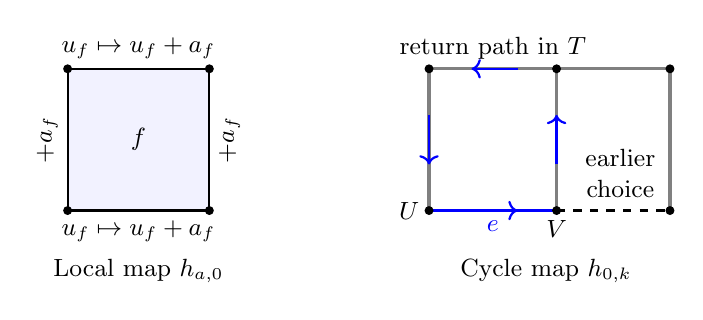
\begin{tikzpicture}[scale=.9, every node/.style={font=\small}]
  \begin{scope}
    \fill[blue!5] (0,0) rectangle (2,2);
    \draw[thick] (0,0)--(2,0)--(2,2)--(0,2)--cycle;
    \foreach \x/\y in {0/0,2/0,2/2,0/2}
      \fill (\x,\y) circle (1.8pt);
    \node at (1,1) {$f$};
    \node[below] at (1,0) {$u_f\mapsto u_f+a_f$};
    \node[above] at (1,2) {$u_f\mapsto u_f+a_f$};
    \node[rotate=90,above] at (0,1) {$+a_f$};
    \node[rotate=90,below] at (2,1) {$+a_f$};
    \node at (1,-.85) {Local map $h_{a,0}$};
  \end{scope}
  \begin{scope}[xshift=5.1cm]
    \coordinate (u) at (0,0);
    \coordinate (v) at (1.8,0);
    \coordinate (a) at (0,2);
    \coordinate (b) at (1.8,2);
    \coordinate (c) at (3.4,2);
    \coordinate (d) at (3.4,0);
    \draw[very thick,gray] (u)--(a)--(b)--(v);
    \draw[very thick,gray] (b)--(c)--(d);
    \draw[thick,blue] (u)--(v);
    \draw[thick,dashed] (v)--(d);
    \draw[->,blue,thick] (.6,0)--(1.25,0);
    \draw[->,blue,thick] (1.8,.65)--(1.8,1.35);
    \draw[->,blue,thick] (1.25,2)--(.6,2);
    \draw[->,blue,thick] (0,1.35)--(0,.65);
    \foreach \p in {u,v,a,b,c,d}
      \fill (\p) circle (1.8pt);
    \node[left] at (u) {$U$};
    \node[below] at (v) {$V$};
    \node[below,blue] at (.9,0) {$e$};
    \node[above] at (.9,2) {return path in $T$};
    \node[above,align=center] at (2.7,.05) {earlier\\choice};
    \node at (1.65,-.85) {Cycle map $h_{0,k}$};
  \end{scope}
\end{tikzpicture}

 \caption{The two parts of a candidate transport.  Left: a translation
 on one face adds the same vector $a_f$ to its four sides and acts on
 their endpoint configurations; the construction uses at most four
 such faces.  The left panel shows only vector coordinates; the scalar
 correction for $h_{a,0}$ is given in
 Equation~\eqref{grid:post-local-scalar}.  Right: the new edge $e$ (blue)
 and its return path in $T$ carry a circulation.  Other tree edges are grey; a previously
 selected edge outside $T$ is dashed and is untouched by the
 circulation.  The picture shows only the relevant part of the tree.}
 \label{grid:figure}
\end{figure}

\subsection{Extending a terminal selection}

Proposition~\ref{grid:transitivity} shows that the output test always
receives a complete, compatible assignment outside its tree.  To
evaluate that test, we must determine whether the remaining edge
states can satisfy all vertex equations.  The vector coordinates
extend face by face; the scalar equations reduce to divergence on a
tree.

\begin{lemma}[Solving divergence on a tree]\label{grid:tree-divergence}
Let $T$ be a finite tree on vertex set $V$, orient its edges arbitrarily,
and write $\partial_T$ for its signed incidence map.  Let $r\in\F^V$
satisfy $\sum_{v\in V}r_v=0$.  There is a unique
$z\in\F^{E(T)}$ with $\partial_T z=r$.
\end{lemma}
\begin{proof}
For a one-vertex tree, the sum condition says $r=0$, and the empty edge
assignment is the unique solution.  Otherwise let $v$ be a leaf, $h$
its incident edge, and $w$ its neighbor.  The equation at $v$ forces
$z_h=\epsilon_{vh}^{-1}r_v$.  Delete $v$ and $h$; keep all other
required divergences except that at $w$, where set
\[
 r'_w=r_w-\epsilon_{wh}z_h=r_w+r_v.
\]
The new required divergences still sum to zero.  Induction supplies
the unique solution on the smaller tree, which together with the
forced value on $h$ solves all the original equations.  Each deleted
edge was forced, proving uniqueness as well.
\end{proof}

\begin{theorem}[Opposite grid answers]\label{grid:separation}
For every $L\ge2$, the fixed sentence $\Phi$ of
Section~\ref{sec:sentence} evaluates to true on $A_{b^0}$ and to false
on $A_{b^1}$.  For either structure, every parameter $\alpha\in P$
and every terminal selection gives the stated output value, and no
evaluation produces $\dagger$.
\end{theorem}
\begin{proof}
By Lemma~\ref{grid:parameters}, both inputs pass the check and have a
nonempty parameter set.  Fix any $\alpha\in P$ and any terminal
selection $x$.  Proposition~\ref{grid:transitivity} says that $x$ is a
complete compatible assignment on the edges outside $T=T(\alpha)$.

First work in $A_{b^0}$.  For each elementary face $f$, choose its
vector $v_f\in\F^2$ to be the one already prescribed by $x$ if an
edge of $f$ was selected, and choose any vector otherwise.
Compatibility makes each prescription unambiguous.  Give every edge
$e$ the vectors $(v_f)_{f\in F(e)}$.  This preserves all selected
vector coordinates and satisfies all face agreements at vertices.

Keep the selected scalars $z_e$ on $e\notin T$, and define the
divergence still required from tree edges by
\[
 r_v=b^0_v-\sum_{e\notin T}\epsilon_{ve}z_e.
\]
Every edge contributes once with each sign, and $\sum_v b^0_v=0$;
therefore $\sum_v r_v=0$.  Lemma~\ref{grid:tree-divergence} supplies
the scalars on $T$.  The resulting full edge assignment has divergence
$b^0$ and satisfies every face agreement.  Its incident tuple at each
vertex is consequently a configuration atom, and neighboring tuples
specify the same edge atom.  By Lemma~\ref{sen:tree-test}, the output
test accepts $x$.

Now work in $A_{b^1}$.  If the output test accepted $x$,
Lemma~\ref{sen:tree-test} would supply configurations agreeing on a
single atom on every edge.  Let $z_e$ denote the scalar of that common
atom.  The equations at all vertices would give
\[
 1=\sum_{v\in V_L}b^1_v
   =\sum_{v\in V_L}\sum_{e\in E_L}\epsilon_{ve}z_e
   =\sum_{e\in E_L}(1-1)z_e=0
 \quad\text{in }\F,
\]
a contradiction.  Thus every terminal selection is rejected.

The witness and resource conclusions of
Proposition~\ref{sen:all-input} apply to these calls, so their values are
Boolean.  The output value just proved is the same for every terminal
selection for each parameter.  Since $P$ is nonempty, the outer
existential aggregation defining $\Phi$ is true on $A_{b^0}$ and false
on $A_{b^1}$, as asserted.
\end{proof}

\section{Small orbits give supports at every rank}\label{sec:support}\label{sup:support}

We now begin the lower-bound argument. The group $H$ of automorphisms from
Section~\ref{str:structures} has an abelian quotient of face translations
and a central subgroup $K$ of edge circulations. Commutators connect these
two parts. We use that connection to show that an object with a small
$H$-orbit is fixed by the pointwise stabilizer in $K$ of a short tuple of
atoms. The bound does not depend on the object's rank. We give the full
support argument from~\cite[Section~3, Proposition~8]{cptCompanion2026}.

Fix $L\ge2$ and $b\in\F^{V_L}$. Write $V=V_L$, $E=E_L$, $F=F_L$,
and $N=|A_b|$. Recall the incidence map
$\partial:\F^E\to\F^V$, the oriented face boundaries $c^f$, and
\[
 K=\ker\partial,\qquad C_F=(\F^2)^F,
 \qquad H=C_F\times K
\]
with the group law of Section~\ref{str:structures}. We identify $K$ with
the central subgroup $\{0\}\times K$ of $H$. Its action fixes face
coordinates and adds $k_e$ to the scalar coordinate of every edge atom
on $e$. As usual, an atom permutation acts on finite sets recursively by
$h\cdot x=\{h\cdot y:y\in x\}$.

\begin{definition}\label{sup:definition}
For an atom tuple $\alpha=(\alpha_1,\ldots,\alpha_r)$, let
\[
 K_\alpha=\{k\in K:k\cdot\alpha_j=\alpha_j
                         \text{ for every }1\le j\le r\}.
\]
The tuple $\alpha$ is a \emph{$K$-support} of an atom or hereditarily
finite set $x$ over $A_b$ if every element of $K_\alpha$ fixes $x$.
The empty tuple is permitted, and $K_{()}=K$.
\end{definition}

The proof has two steps. First, an edge functional whose curl is nonzero
on few faces can be represented on few edges. Second, the small index of
an object's stabilizer forces precisely this curl condition for the
functionals that detect its central stabilizer.

\subsection{Sparse representatives of edge functionals}

An \emph{edge cochain} is a vector $\ell\in\F^E$. Define its curl
$D\ell\in\F^F$ by
\[
 (D\ell)(f)=\sum_{e\in E}c^f_e\ell_e.
\]
For a vertex function $\varphi\in\F^V$, its gradient is
$\partial^{\mathsf T}\varphi$; on an edge directed from $v$ to $w$ it
has value $\varphi(w)-\varphi(v)$. Since $\partial c^f=0$, adding a
gradient changes neither the curl nor the functional
$k\mapsto\sum_e\ell_e k_e$ on $K$.

\begin{lemma}[Sparse cochains]\label{sup:sparse-cochain}
Let $\ell\in\F^E$, and let
$t=|\{f\in F:(D\ell)(f)\ne0\}|$. There is a vertex function
$\varphi\in\F^V$ such that
\[
 |\operatorname{supp}(\ell-\partial^{\mathsf T}\varphi)|\le2Lt,
 \qquad
 \operatorname{supp}(r)=\{e\in E:r_e\ne0\}.
\]
In particular, every cochain with zero curl is a gradient.
\end{lemma}

\begin{proof}
We first eliminate the cochain in one coordinate direction. We then
eliminate a second direction on a slice containing few nonzero curls,
and use the remaining curls to bound the support away from that slice.

Write vertices as $(i,j,k)$. The coordinate $\ell_1(i,j,k)$ belongs to
the edge from $(i,j,k)$ to $(i+1,j,k)$, and $\ell_2,\ell_3$ are defined
similarly. A direction-$a$ edge coordinate is used only when increasing
coordinate $a$ stays in the box. Put
\[
 \varphi_1(i,j,k)=\sum_{u=0}^{i-1}\ell_1(u,j,k),
 \qquad r^{(1)}=\ell-\partial^{\mathsf T}\varphi_1,
\]
where empty sums are zero. Then $r^{(1)}_1=0$. The face orientation
$+1,+a,-1,-a$ gives
\begin{align}
 (D\ell)_{12}(i,j,k)
   &=r^{(1)}_2(i+1,j,k)-r^{(1)}_2(i,j,k),\label{sup:curl12}\\
 (D\ell)_{13}(i,j,k)
   &=r^{(1)}_3(i+1,j,k)-r^{(1)}_3(i,j,k).\label{sup:curl13}
\end{align}
Here $ab$ indicates the face in directions $a<b$ with lower corner
$(i,j,k)$, and the identity is asserted whenever that face exists.

Let $t_{ab}$ be the number of nonzero $ab$ curls, so
$t=t_{12}+t_{13}+t_{23}$. The $23$ faces are partitioned into the $L$
slices of fixed first coordinate. Choose a slice $i=i_0$ containing
$t_0\le t_{23}/L$ nonzero $23$ curls. Define
\[
 \varphi_2(i,j,k)=\sum_{v=0}^{j-1}r^{(1)}_2(i_0,v,k),
 \qquad r^{(2)}=r^{(1)}-\partial^{\mathsf T}\varphi_2.
\]
Because $\varphi_2$ is independent of $i$, we still have
$r^{(2)}_1=0$, and now $r^{(2)}_2(i_0,j,k)=0$. Finally put
\[
 \varphi_3(i,j,k)=\sum_{w=0}^{k-1}r^{(2)}_3(i_0,0,w),
 \qquad r=r^{(2)}-\partial^{\mathsf T}\varphi_3.
\]
The function $\varphi_3$ is independent of $i,j$, so
\[
 r_1=0,\qquad r_2(i_0,j,k)=0,\qquad r_3(i_0,0,k)=0.
\]
All three gradient subtractions preserve curl. On the selected slice
the $23$ curl identity therefore becomes
\[
 r_3(i_0,j+1,k)-r_3(i_0,j,k)=(D\ell)_{23}(i_0,j,k).
\]
For each fixed $k$, every nonzero value of $r_3(i_0,j,k)$ has a nonzero
curl earlier on its $j$-line. One nonzero curl can affect at most $L$
positions on that line. Thus at most $Lt_0$ direction-$3$ edge
coordinates on the slice are nonzero. Direction $2$ is zero there.

Copy these direction-$2$ and direction-$3$ slice values to every first
coordinate $i$, obtaining a reference cochain supported on at most
$L^2t_0$ edges, with direction $1$ zero. Identities
\eqref{sup:curl12} and~\eqref{sup:curl13} remain valid for $r$.
Consequently
\[
 r_2(i,j,k)-r_2(i_0,j,k)
\]
is the signed sum of the $12$ curls between $i_0$ and $i$ on that line.
A nonzero $12$ curl occurs in at most $L$ such sums, so at most
$Lt_{12}$ direction-$2$ coordinates differ from the reference cochain.
The same reasoning bounds the differing direction-$3$ coordinates by
$Lt_{13}$. A coordinate in the support of $r$ must either belong to
the reference support or differ from its reference value. Hence
\[
 |\operatorname{supp}(r)|
 \le L^2t_0+L(t_{12}+t_{13})\le Lt\le2Lt.
\]
Taking $\varphi=\varphi_1+\varphi_2+\varphi_3$ proves the claim. The
same construction gives $r=0$ when $t=0$.
\end{proof}

\subsection{From a small orbit to a support}

\begin{proposition}[Small-orbit support bound]\label{sup:small-orbit}
Let $L\ge2$, $b\in\F^{V_L}$, and $N=|A_b|$. Let $q\ge0$ and let $x$
be an atom or a hereditarily finite set over $A_b$. If
$|H\cdot x|\le N^q$, then $x$ has a $K$-support consisting of at most
\[
 2L(q\log_3N)^2
\]
edge atoms. There is no bound on the finite rank of $x$ in this statement.
\end{proposition}

\begin{proof}
Let $S=\{h\in H:h\cdot x=x\}$ be the stabilizer of $x$. Let $U$ be
its image under the projection $H\to C_F$, and put $K_0=S\cap K$.
Both $U$ and $K_0$ are subgroups of additive groups over the prime field
$\F$, and hence are vector subspaces. Define
\[
 a=\operatorname{codim}_{C_F}U,\qquad
 d=\operatorname{codim}_{K}K_0,\qquad
 h=\log_3[H:S].
\]
The restriction of the projection to $S$ has image $U$ and kernel $K_0$.
Every fibre has size $|K_0|$, so $|S|=|U|\,|K_0|$. Since
$|H|=|C_F|\,|K|$, orbit--stabilizer gives
\begin{equation}\label{sup:index}
 a+d=h=\log_3|H\cdot x|\le q\log_3N.
\end{equation}

Consider the annihilator
\[
 W=\{\lambda\in K^*: \lambda(k)=0\text{ for all }k\in K_0\},
 \qquad \dim W=d,
\]
where $K^*$ is the linear dual of $K$. Each $\lambda\in K^*$ extends
to a linear functional on $\F^E$: extend a basis of $K$ to one of
$\F^E$ and assign arbitrary values on the additional basis vectors.
The standard coordinate pairing thus gives an edge cochain $\ell$ with
\[
 \lambda(k)=\sum_{e\in E}\ell_e k_e\quad(k\in K).
\]
Two representatives differ by an element of
$K^\perp=\operatorname{im}\partial^{\mathsf T}$. Indeed the latter
space is contained in $K^\perp$, and both have dimension
$\operatorname{rank}\partial$. In particular, their curls agree.

Fix $\lambda\in W$ and a representative $\ell$. For any $u,u'\in U$,
choose lifts in $S$. Their commutator belongs to $K_0$; the commutator
formula~\eqref{str:commutator} therefore implies
\begin{equation}\label{sup:isotropic}
 0=\sum_{f\in F}(D\ell)(f)\,\omega(u_f,u'_f).
\end{equation}
The right-hand side defines an alternating bilinear form $\beta_\ell$
on $C_F$. If $t$ of the coefficients $(D\ell)(f)$ are nonzero, its
rank is $2t$: each nonzero coefficient multiplies a nondegenerate
two-dimensional alternating block, and the face coordinates are
independent summands of $C_F$. Relations among the boundary vectors
$c^f$ do not identify these summands.

We use the standard dimension bound for isotropic subspaces of an
alternating form, after quotienting by its radical
\cite[Sections~3.1 and~3.3]{cameron2000classical}.
Equation~\eqref{sup:isotropic} says that $U$ is totally isotropic for
$\beta_\ell$, meaning that the form vanishes on $U\times U$. Put
$n_F=\dim C_F$, and let
$R=\{v\in C_F:\beta_\ell(v,w)=0\text{ for every }w\in C_F\}$
be the radical of this form. The quotient $C_F/R$ is nondegenerate of
dimension $2t$. The image $\overline U$ of $U$
is isotropic, so $\overline U\subseteq\overline U^{\perp}$ and
$\dim\overline U\le t$. The radical has dimension $n_F-2t$, whence
\[
 \dim U\le(n_F-2t)+t=n_F-t,
 \qquad t\le a.
\]
Lemma~\ref{sup:sparse-cochain} now replaces $\ell$ by a representative
of the same functional $\lambda$ supported on at most $2La$ edges.

We have obtained a sparse representative for every functional detecting
the quotient $K/K_0$. Choose such representatives for a basis of $W$,
and let $T\subseteq E$ be the union of their supports. Then
\begin{equation}\label{sup:edge-support-size}
 |T|\le2Lad\le2Lh^2\le2L(q\log_3N)^2.
\end{equation}
When $d=0$, use the empty basis and $T=\emptyset$. If $k\in K$
vanishes on $T$, every member of that basis vanishes on $k$. Thus all
of $W$ vanishes on $k$, and finite-dimensional duality gives $k\in K_0$.
For each $e\in T$, choose one edge atom on $e$, and list the chosen
atoms in a tuple $\alpha$. The central action in
\eqref{str:edge-action} fixes that atom exactly when $k_e=0$.
Consequently $K_\alpha\subseteq K_0\subseteq S$, so $\alpha$ supports
$x$ and satisfies~\eqref{sup:edge-support-size}. This argument concerns
the stabilizer of $x$ alone and makes no induction on its rank.
\end{proof}

\subsection{Hereditary support for finite invariant families}

A family $\mathcal X$ of atoms and hereditarily finite sets is
\emph{membership-transitive} if $y\in x\in\mathcal X$ implies
$y\in\mathcal X$. It then contains every object reached from a member
by any finite sequence of membership steps. We call an object
\emph{hereditarily $s$-supported} if it and every such recursive member
have a $K$-support of length at most $s$; these supports need not coincide.

\begin{corollary}\label{sup:hereditary}
Let $L\ge2$, $b\in\F^{V_L}$, and $N=|A_b|$. Suppose $\mathcal X$ is
a finite $H$-invariant, membership-transitive family of atoms and
hereditarily finite sets over $A_b$, with $|\mathcal X|\le N^q$ for
some $q\ge0$. Every member of $\mathcal X$ and every recursive member
has a $K$-support of length at most $2L(q\log_3N)^2$. In particular,
every member is hereditarily $s$-supported for
\begin{equation}\label{sup:length}
 s=\left\lceil2L(q\log_3N+1)^2\right\rceil+1.
\end{equation}
All the supports may be padded to length exactly $s$. For fixed $q$,
\[
 s=O_q\bigl(L(1+\log L)^2\bigr).
\]
\end{corollary}

\begin{proof}
$H$-invariance places the orbit of each $x\in\mathcal X$ inside
$\mathcal X$. Proposition~\ref{sup:small-orbit} therefore gives the
claimed support for every member. Membership transitivity gives the
same conclusion for all recursive members. Adding coordinates to an
atom tuple can only shrink its pointwise stabilizer, so it preserves
the support property. Since $L\ge2$, the base has an edge atom; append
copies of any one such atom to reach length $s$, including when the
original support is empty. Finally Lemma~\ref{str:size} gives
$N=\Theta(L^3)$, which yields the displayed asymptotic bound.
\end{proof}

\section{Counting equivalence and central-group homogeneity}
\label{sec:base-counting}
\label{base:counting}

We now establish the two facts about atom tuples needed to transfer
supports.  With sufficiently few variable names, counting logic cannot
distinguish the zero-charge and unit-charge structures.  Within either
structure, however, the counting type of a short tuple determines its
orbit under the central group $K=\ker\partial$.  Both statements will be
proved in an auxiliary expansion of the structures from
Section~\ref{str:structures}.  We give the quantitative base argument
from~\cite[Section~4, Propositions~11 and~13]{cptCompanion2026} in full.

Throughout this section, write $V=V_L$, $E=E_L$, and let $G=(V,E)$ denote
the undirected box graph, retaining the fixed edge orientations when
using $\partial$.  Thus an element $k\in K$ adds $k_e$ to the scalar
coordinate of every state on $e$, and acts on configurations by the
induced changes of their incident states.

\subsection{The auxiliary expansion and counting types}

Partition the atoms of $A_b$ into classes with labels
\[
 (e,u),\qquad
   e\in E,\quad u\in(\F^2)^{F(e)},
 \qquad\text{and}\qquad
 (v,\eta),\qquad
   v\in V,\quad \eta\in(\F^2)^{F(v)}.
\]
An edge class consists of the three atoms $(e,u,z)$ with its indicated
$e,u$.  A configuration class consists of the configurations at $v$
whose common vector on each face $f\in F(v)$ is $\eta_f$.  The latter
class has $3^{\deg(v)-1}$ members: its scalar coordinates satisfy just
the one divergence equation.  Every class is therefore nonempty, and
its size is independent of $b$.

Choose a linear order of these labels, using the same order for all
charge assignments at a fixed $L$.  Add the binary relation $\preceq$
which compares atoms by their labels, so that its equivalence classes
are exactly the classes just defined.  Also add three binary relations
$\mathsf D_\delta$, for $\delta\in\F$, given by
\[
 \mathsf D_\delta\bigl((e,u,z),(e',u',z')\bigr)
 \quad\Longleftrightarrow\quad
 e=e'\ \text{ and }\ z'-z=\delta.
\]
They are false on pairs involving a configuration atom.  The vector
patterns $u,u'$ need not be equal.  Denote the expansion by $\bar A_b$.
Its vocabulary is still fixed and binary.  Every element of $K$
preserves it, since central translations fix the labels and preserve
raw scalar differences.  The group $H$ is only required to act on the
original input; these additional relations are used in the proof and
are never supplied to a choiceless program.

For a positive integer $h$, let $C^h$ be first-order logic with equality,
ordinary quantifiers, and exact counting quantifiers
$\exists^{=a}x$, using at most $h$ distinct variable names.  The formula
$\exists^{=a}x\,\varphi$ is true precisely when exactly $a$ elements
satisfy $\varphi$, where $a$ is any nonnegative integer.  Formula length
and counting constants are unrestricted.  In particular, when comparing
structures for a fixed $L$, the formulas may depend on $L$.

For an $r$-tuple $\bar a$ with $r\le h$, its $C^h$-type is the set of
all $C^h$ formulas true at $\bar a$ whose free variables belong to its
$r$ designated positions.  The positions have distinct variable names,
but their assigned atoms may repeat.  Types on different structures are
compared using the same designated positions.

\subsection{A large component after deleting few edges}

Write $\delta_G R$ for the edge boundary of a vertex set $R\subseteq V$;
this is separate from the incidence map $\partial$.  We first show that
a small set of deleted edges cannot split the box into small pieces.
The projection step is the three-dimensional discrete Loomis--Whitney
inequality~\cite{loomisWhitney1949}; its short proof below
also gives the finite-box boundary constant needed here.

\begin{lemma}[Boundary estimate]
\label{base:boundary}
Let $c=1-2^{-1/3}$.  For every $L\ge2$ and every nonempty
$R\subseteq\{0,\ldots,L-1\}^3$ with $|R|\le L^3/2$,
\[
 |\delta_G R|\ge c|R|^{2/3}.
\]
\end{lemma}
\begin{proof}
Let $a_{ij},b_{ik},d_{jk}$ be the indicators of the three projections of
$R$ onto coordinate pairs, and let their sizes be $A,B,D$, respectively.
Every point of $R$ contributes to the product of these indicators.
Twice applying Cauchy--Schwarz gives
\begin{align*}
 |R|
 &\le\sum_{i,j,k}a_{ij}b_{ik}d_{jk}\\
 &\le A^{1/2}
      \left(\sum_{i,j}\left(\sum_k b_{ik}d_{jk}\right)^2\right)^{1/2}
 \le (ABD)^{1/2}.
\end{align*}
For the last step, bound each squared inner sum by
$(\sum_k b_{ik}^2)(\sum_k d_{jk}^2)$ and then sum over $i,j$.
At least one projection consequently has size at least $|R|^{2/3}$.
It indexes that many nonempty coordinate lines meeting $R$.  At most
$|R|/L$ of these lines lie wholly in $R$.  Each of the remaining lines
is a path meeting both $R$ and its complement, and hence contains a
boundary edge.  The lines are disjoint, so these edges are distinct.
Finally,
\[
 |\delta_G R|\ge |R|^{2/3}-\frac{|R|}{L}
 \ge (1-2^{-1/3})|R|^{2/3},
\]
where the last inequality uses $|R|\le L^3/2$.
\end{proof}

Set
\begin{equation}
\label{base:M}
 M=\lfloor L^{7/4}\rfloor.
\end{equation}

\begin{lemma}[Persistent large component]
\label{base:giant}
For all sufficiently large $L$, every graph $G\setminus T$ obtained by
deleting at most $6M$ edges has a unique component with more than
$L^3/2$ vertices.  If $T\subseteq T'$ and $|T'|\le6M$, the component
for $T'$ is contained in the component for $T$.
\end{lemma}
\begin{proof}
Sum Lemma~\ref{base:boundary} over the components $R$ of $G\setminus T$
having at most $L^3/2$ vertices.  Every boundary edge belongs to $T$
and is counted at most twice.  Thus
\begin{equation}
\label{base:small-components}
 \sum_R |R|
 \le c^{-3/2}\sum_R|\delta_G R|^{3/2}
 \le c^{-3/2}(2|T|)^{3/2}
 \le c^{-3/2}(12M)^{3/2}=o(L^3).
\end{equation}
Here $\sum_j a_j^{3/2}\le(\sum_j a_j)^{3/2}$ for nonnegative $a_j$,
and $M^{3/2}=O(L^{21/8})=o(L^3)$.  If every component had at most half
the vertices, the left side would be $L^3$, a contradiction for large
$L$.  Two components cannot both contain more than half the vertices.
After further deletion each component is contained in an old component;
its size forces the new large component to lie in the old large one.
\end{proof}

We call the component in Lemma~\ref{base:giant} the \emph{giant
component}.  The next proof uses it to keep the single unmatched charge
away from all assigned atoms.  Its extension step constructs a bijection
of the entire universes, which is what exact counting requires.

\subsection{Counting equivalence of the two charge assignments}

The argument adapts the defect-moving method of the CFI construction
\cite[Section~6]{cfi1992} and the finite-variable counting-game method
of Immerman and Lander~\cite[Counting Quantifiers]{immermanLander1990}.
We construct whole-universe bijections and prove formula preservation
directly, so no game characterization is an additional premise.

\begin{proposition}[Base counting equivalence]
\label{base:equivalence}
For all sufficiently large $L$, the expansions $\bar A_{b^0}$ and
$\bar A_{b^1}$ satisfy the same $C^M$ sentences, where
$b^0=0$, $b^1=\mathbf1_{v_*}$, and $M$ is as in
\eqref{base:M}.
\end{proposition}
\begin{proof}
An assigned edge atom \emph{touches} its edge.  An assigned configuration
atom at $v$ touches every edge incident with $v$.  The edges touched by
at most $M$ assigned positions form a set $T$ of size at most $6M$.

Call paired assignments in the two structures \emph{compatible} if they
have matching block and vector labels and there exist $t\in\F^E$ and
a vertex $w$ in the giant of $G\setminus T$ such that
\begin{equation}
\label{base:defect}
 \partial t=b^1-b^0-\mathbf1_w,
\end{equation}
and each atom in the first assignment is paired with the atom obtained
by adding $t_e$ on every incident scalar coordinate.  The empty
assignments are compatible: take $t=0$ and $w=v_*$.

Compatible assignments preserve atomic formulas.  On any fixed edge,
common addition of $t_e$ preserves raw scalar differences, and also the
corrected differences defining each $\Zrel_\delta$, since vector
coordinates do not change.  It preserves whether the assigned edge
atom is the state specified by an assigned configuration.  Blocks,
sorts, the preorder, and equality are likewise preserved, including
when positions have repeated values.  An assigned configuration cannot
be at $w$: deleting its whole star isolates its vertex, whereas $w$
lies in a component with more than half the vertices.  Thus the shift
at every assigned configuration satisfies the appropriate change of
divergence in \eqref{base:defect}.

Forgetting an assigned position preserves compatibility.  Its touched
edges may disappear from $T$, and Lemma~\ref{base:giant} places the old
giant inside the new one.  Suppose now that at most $M-1$ positions
remain.  We construct a bijection of universes which retains their
pairings and gives a compatible extension for every possible next atom.

Partition the atoms into whole edge blocks and whole configuration
blocks.  For each such block $J$, let $T_J$ be $T$ together with the
edge of $J$, or the star of its vertex, respectively.  Then
$|T_J|\le6M$.  Choose a vertex $w_J$ in the giant of $G\setminus T_J$.
By Lemma~\ref{base:giant}, both $w$ and $w_J$ lie in the giant of
$G\setminus T$.  Choose a signed path vector $p_J$ supported outside
$T$ with
\[
 \partial p_J=\mathbf1_w-\mathbf1_{w_J};
\]
one may traverse a path from $w_J$ to $w$, or use zero if they agree.
The vector $t_J=t+p_J$ agrees with $t$ on $T$ and satisfies
\eqref{base:defect} with $w_J$ in place of $w$.

On the block $J$, map every atom by its $t_J$-shift.  For an edge block
this is plainly a bijection to the corresponding block.  For a
configuration block at $v$, deleting its star isolates $v$, so
$v\ne w_J$.  Therefore
\[
 (\partial t_J)_v=b^1_v-b^0_v,
\]
which is exactly the condition making translation a bijection between
the two configuration blocks.  All their vector constraints stay the
same.  Taking the union over the disjoint blocks gives a bijection of
the whole universes.  On every retained assignment it agrees with the
old pairing because $p_J$ vanishes on $T$.  If the next atom belongs
to $J$, the extended assignment has witness $t_J,w_J$: its touched
set is $T_J$, and all retained coordinates still have the right images.

Induct on formulas to show that compatible assignments agree on every
$C^M$ formula with their designated free positions.  Atomic formulas
were checked above; Boolean connectives preserve agreement.  At a
quantifier, forget the old value, if any, of its bound variable.  At
most $M-1$ positions remain.  The universe bijection just constructed
pairs extensions with compatible assignments, so induction makes the
body true on equally many extensions.  It preserves ordinary
quantifiers and every exact counting quantifier, including count zero.
Apply this conclusion to the empty assignments.
\end{proof}

\subsection{Extending partial central translations}

For homogeneity, both tuples lie in the same expansion $\bar A_b$.
Their coordinates will prescribe a scalar translation on the touched
edges.  We first identify exactly when it extends to an element of $K$.

\begin{lemma}[Partial-flow extension]
\label{base:partial-flow}
Let $T\subseteq E$ and $\sigma\in\F^T$.  There is a vector
$k\in\ker\partial$ with $k|_T=\sigma$ if and only if every component
$U$ of $G\setminus T$ satisfies
\begin{equation}
\label{base:balance}
 R_U:=\sum_{v\in U}\sum_{\substack{e\in T\\e\ni v}}
          \epsilon_{ve}\sigma_e=0.
\end{equation}
If no extension exists, some nonempty component violating
\eqref{base:balance} has
\[
 |U|\le L^3/2,
 \qquad |U|\le(|T|/c)^{3/2}.
\]
\end{lemma}
\begin{proof}
Extend $\sigma$ by zero to all of $E$.  An extension is equivalent to
a vector on $E\setminus T$ having divergence $-\partial\sigma$.
On a connected graph, an incidence vector always has total sum zero.
Conversely, any specified vertex vector of total sum zero is an
incidence vector: choose a spanning tree, give nontree edges value zero,
and remove leaves successively.  The equation at a leaf determines its
tree-edge value uniquely because its coefficient is $1$ or $-1$.
The total-sum condition makes the last root equation hold.  This also
handles a one-vertex component, where the only possible divergence is
zero.  Applied separately to each component of $G\setminus T$, this
argument gives exactly the conditions \eqref{base:balance}.

The sum of all $R_U$ is zero, since the two incidence signs of each
edge cancel.  If one component fails, at least two fail.  Hence one
failing component has at most $L^3/2$ vertices.  Its boundary is
contained in $T$, so Lemma~\ref{base:boundary} yields
$c|U|^{2/3}\le|\delta_G U|\le|T|$.
\end{proof}

\begin{proposition}[Quantitative $K$-homogeneity]
\label{base:homogeneity}
Let $L\ge2$, $b\in\F^V$, and let $r,M$ be positive integers such that
\begin{equation}
\label{base:homogeneity-bound}
 7r+7(6r/c)^{3/2}+1\le M.
\end{equation}
If two $r$-tuples in $\bar A_b$ have the same $C^M$-type, an element
of $K$ maps the first tuple to the second.  Empty tuples lie in the
same $K$-orbit without any width hypothesis.
\end{proposition}
\begin{proof}
Write the tuples as $\bar a,\bar a'$.  The proof first extracts a
consistent scalar shift on the touched edges, then uses a formula to
exclude every obstruction from Lemma~\ref{base:partial-flow}.

Each preorder class is defined with two variable names.  If $h$ is the
number of atoms in strictly earlier classes, its predicate is
\begin{equation}
\label{base:class-predicate}
 \theta_h(x):=\exists^{=h}y\,
          (y\preceq x\land\neg(x\preceq y)).
\end{equation}
Different classes have different $h$ because every class is nonempty.
Equality of types therefore places $a_i$ and $a_i'$ in the same class
for every $i$.  In particular, their blocks and complete vector
patterns agree.  The two tuples touch the same set $T$ of edges, with
$|T|\le6r$.

An \emph{occurrence} on $e\in T$ is either an edge atom in a tuple
position, or the state on $e$ specified by a configuration in a tuple
position.  In the latter case this state is the unique atom $y$ such
that $\Inc(a_i,y)$ holds and $y$ has its specified edge-class label.
The label includes $e$ and the vector pattern, so it is expressed by
one of the predicates \eqref{base:class-predicate}.  Corresponding
occurrences for $\bar a$ and $\bar a'$ consequently have the same
edge and vector coordinates.

For two occurrences on the same edge, their raw scalar difference is
testable using $\mathsf D_\delta$, introducing their uniquely specified
neighbors when necessary.  Such a test uses at most the $r$ tuple
names, two neighbor names, and one further name reused in class
predicates.  Inequality~\eqref{base:homogeneity-bound} supplies these
$r+3$ names.  The raw differences of corresponding occurrences are
therefore equal.  It follows that for every $e\in T$ there is a single
well-defined value $\sigma_e\in\F$: the scalar change from an
occurrence in $\bar a$ to its counterpart in $\bar a'$.  The value is
independent of the chosen occurrence.

Suppose this partial shift $\sigma$ does not extend to $K$.  By
Lemma~\ref{base:partial-flow}, a component $U$ of $G\setminus T$ has
\[
 R_U\ne0,\qquad |U|\le(6r/c)^{3/2}.
\]
We construct a formula distinguishing $\bar a$ from $\bar a'$ within
the stated variable bound.

Choose, for each $v\in U$, an arbitrary configuration atom $g_v^0$ in
$\bar A_b$, and denote its state on an incident edge $e$ by
$h_{v,e}^0$.  Such configurations exist for every $v$.  On each boundary
edge $e\in\delta_G U\subseteq T$, choose one tuple occurrence and
write its state as $o_e^0$.  Let $z(s)$ denote the scalar coordinate of
an edge state $s$; in the following construction it is only used to
specify one of the three relation symbols $\mathsf D_\delta$.

The formula existentially quantifies a configuration variable $g_v$
for each $v\in U$, a state variable $h_{v,e}$ for every edge incident
with $v$, and, when $o_e^0$ comes from a tuple configuration, one
additional neighbor variable $y_e$.  Write $o_e$ for this $y_e$ or for
the selected tuple variable when the occurrence is already an edge
atom.  The conjunction under these quantifiers imposes the following
conditions:
\begin{enumerate}
\item Each $g_v$ and $h_{v,e}$ has the class of its reference atom
      $g_v^0$ or $h_{v,e}^0$, and $\Inc(g_v,h_{v,e})$ holds.
\item On every edge $e$ with both endpoints $v,w\in U$, choose one
      ordering of the endpoints and impose
      \[
       \mathsf D_{z(h_{w,e}^0)-z(h_{v,e}^0)}
                (h_{v,e},h_{w,e}).
      \]
\item On every boundary edge $e$ with endpoint $v\in U$, impose
      \[
       \mathsf D_{z(h_{v,e}^0)-z(o_e^0)}(o_e,h_{v,e}).
      \]
      When $o_e=y_e$, also require its reference edge class and its
      incidence with the chosen tuple configuration.
\end{enumerate}
All class conditions use \eqref{base:class-predicate}.  Thus this is
a finite formula in the expansion's vocabulary, with $\bar a$ as
its free assignment.  Its length and counting constants may depend
on the chosen reference atoms.  The reference configurations and
states witness that it is true at $\bar a$.

The internal-edge condition also applies when $e\in T$ has both
endpoints in $U$.  It does not link that edge to a tuple occurrence;
the two contributions of such an edge to $R_U$ already cancel.  Also,
the reference configurations need not have matching vector patterns
on their common edge.  This is why $\mathsf D_\delta$ was defined
between all states on the same edge, irrespective of their vectors.

If the formula were true at $\bar a'$, compare its state witnesses to
the reference states and put
\[
 d_{v,e}=z(h_{v,e})-z(h_{v,e}^0).
\]
Both configurations at $v$ have divergence $b_v$, so
\[
 \sum_{e\ni v}\epsilon_{ve}d_{v,e}=0.
\]
The constraints on an internal edge give $d_{v,e}=d_{w,e}$.  On a
boundary edge, the tuple occurrence has scalar change $\sigma_e$;
its uniqueness also gives this change when it is represented by
$y_e$.  The boundary constraint therefore forces
$d_{v,e}=\sigma_e$.  Summing the displayed vertex equations over $U$
cancels every internal edge and leaves $R_U=0$, a contradiction.

To count variable names, retain the $r$ tuple names, use $|U|$
configuration names and at most $6|U|$ incident-state names, and use
at most $|\delta_G U|\le6r$ extra occurrence names.  One additional
name can be reused inside every class predicate without capturing
any of these names.  The total is at most
\[
 r+7|U|+6r+1
 \le7r+7(6r/c)^{3/2}+1\le M.
\]
We have obtained a $C^M$ formula distinguishing the tuples, contrary
to their type equality.  Hence $\sigma$ extends to some $k\in K$.
Its action maps each edge occurrence, and thus every tuple
configuration as well, to its counterpart.  For empty tuples, take
$k=0$.
\end{proof}

The support scale from the preceding section is much smaller than the
width available here.  We record the comparison with all parameters
fixed in the order needed later.

\begin{corollary}[Widths at the support scale]
\label{base:width}
Fix positive integers $q,m$ independently of $L$, and let
\[
 N=N_L=\Theta(L^3),\qquad
 s=\left\lceil2L(q\log_3N+1)^2\right\rceil+1,
 \qquad M=\lfloor L^{7/4}\rfloor.
\]
For all sufficiently large $L$, Proposition~\ref{base:equivalence}
holds, Proposition~\ref{base:homogeneity} applies to every tuple length
$1\le r\le(m+4)s$ in either expansion, and
\[
 \max\{4,m+1\}s\le M.
\]
In particular, both expansions are $K$-homogeneous for equal $C^M$
types of tuples of length at most $\max\{2,m\}s$.
\end{corollary}
\begin{proof}
By $N=\Theta(L^3)$,
$s=O_q(L(1+\log L)^2)$.  Uniformly for $1\le r\le(m+4)s$, the left
side of \eqref{base:homogeneity-bound} is
\[
 O_{q,m}\bigl(L^{3/2}(1+\log L)^3\bigr)=o(L^{7/4}).
\]
The floor in $M$ does not affect this eventual inequality.  Also,
$\max\{4,m+1\}s=o(L^{7/4})$.  Increasing $L$ if necessary supplies
Lemma~\ref{base:giant} and Proposition~\ref{base:equivalence} as well.
The threshold may depend on the fixed $q,m$.
\end{proof}

\section{Counting equivalence at every finite rank}
\label{hf:section}
\label{sec:hf-transfer}

Small supports connect the atom structure with the sets built during a
choiceless computation.  The connection must preserve exact counts, even
though supported objects can have arbitrarily large finite rank.
We prove an abstract transfer theorem for this purpose.  Its proof first
represents supported objects by finite expressions over support tuples,
then compares the finite orbits of those objects after parameters have
been fixed.  Matching these orbits will produce a bijection of the entire
supported domains.
Forms and molecules originate in Blass, Gurevich and Shelah
\cite[Sections~8--9, published version]{bgs1999} and were developed
for counting by Dawar, Richerby and Rossman
\cite[Section~8, Theorem~33, author version]{drr2008}.
Their hereditary-support transfer already permits arbitrary finite rank.
We give the quantitative group-relative version proved in
\cite[Section~5, Theorem~14]{cptCompanion2026}, including its complete
orbit-counting argument.

Let $B$ be a finite relational structure, also writing $B$ for its
universe, and let $K\leq\Aut(B)$.  Regard the elements of $B$ as atoms,
distinct from every set, and extend the action of $K$ recursively to
$\HF(B)$.  A tuple $\alpha$ of atoms \emph{supports} $x\in\HF(B)$ if
every element of $K$ fixing $\alpha$ coordinatewise fixes $x$.
For an integer $s\geq1$, let
\[
 \begin{aligned}
 D_s(B,K)=\{x\in\HF(B):{}&
 \text{$x$ and every recursive member of $x$}\\
 &\text{have a $K$-support of length at most $s$}\}.
 \end{aligned}
\]
Here a recursive member is an object reached by a positive number of
membership steps.  We view $D_s(B,K)$ as a relational structure with
membership, a unary atom predicate, and the relations of $B$, interpreted
as false whenever an argument is a set.  This domain is closed under
taking members and is invariant under $K$.  It contains every atom and
every pure hereditarily finite set, since an atom supports itself and a
pure set has empty support.  Consequently the domain is countably
infinite when $B$ is finite, although each of its individual objects is
hereditarily finite.

For a tuple $\bar a$ of length at most $M$, write
$\operatorname{tp}^{B}_M(\bar a)$ for its complete $C^M$ type:
the set of all $C^M$ formulas true at $\bar a$, with free variables among
the indicated ordered tuple positions.  Tuple entries may repeat.
The variable bound restricts the stock of variable names, not the length
of a formula or the natural-number constants in exact counting
quantifiers.

\begin{theorem}[Transfer through small supports]
\label{hf:transfer}
Let $B_0,B_1$ be nonempty finite structures in the same finite relational
vocabulary of arity at most two, and let
$K_i\leq\Aut(B_i)$ for $i=0,1$.
Let $s,m,M$ be positive integers with
\[
                         \max\{4,m+1\}s\leq M.
\]
Suppose that:
\begin{enumerate}
\item $B_0$ and $B_1$ satisfy the same $C^M$ sentences;
\item in each $B_i$, any two tuples of length at most
      $\max\{2,m\}s$ having the same $C^M$ type belong to the same
      $K_i$-orbit.
\end{enumerate}
Then $D_s(B_0,K_0)$ and $D_s(B_1,K_1)$ satisfy the same $C^m$ sentences
in membership, atomhood, and the base relations.
\end{theorem}

All supports below are padded to length exactly $s$.
This is possible by repeating entries, or by using an arbitrary atom
when the support is empty; the nonemptiness hypothesis is used here.
Padding preserves the support property.  Write
$D_i=D_s(B_i,K_i)$ for the rest of the proof.

\subsection{Exact extension counts of atom types}

Only types realized in $B_0$ or $B_1$ will be used.  For each fixed tuple
length there are finitely many such types.  Although a complete type is
an infinite collection of formulas, its class of realizations in these
two finite structures can be isolated by one finite formula.

\begin{lemma}[Extension counts]
\label{hf:extension-counts}
Let $P,P'$ be tuples of the same length $a$, in two structures chosen
from $B_0,B_1$, allowing the two structures to be the same.
Suppose that $P,P'$ have the same $C^M$ type.
If $a+d\leq M$, then for every realized type $\rho$ of length $a+d$,
the numbers of tuples $\gamma,\gamma'$ of length $d$ satisfying
\[
 \operatorname{tp}_M(P,\gamma)=\rho,
 \qquad
 \operatorname{tp}_M(P',\gamma')=\rho
\]
are equal.  Equal types also give equal types on every projected or
reordered subtuple.
\end{lemma}

\begin{proof}
Projection and reordering follow by renaming variable positions:
an injection from the selected positions to the original positions
extends to a permutation of the $M$ variable names.  This renames bound
variables as well, so it avoids capture.  Repeated atom values cause
no difficulty, because equality formulas record them.

For $d=1$, choose a tuple realizing $\rho$.  For every tuple in either
finite structure whose type differs from $\rho$, choose a formula
distinguishing it from this representative, and negate that formula
if necessary so that the representative satisfies it.  The conjunction
of these finitely many formulas, denoted $\theta_\rho$, holds exactly
on the tuples of type $\rho$ in the two structures.  It has free
variables among the first $a+1$ positions and uses the same $M$ variable
names.  If there are no other types, take a tautology.
If $P$ has exactly $h$ extensions realizing $\rho$, then
\[
       \exists^{=h}x_{a+1}\,
       \theta_\rho(x_1,\ldots,x_a,x_{a+1})
\]
holds at $P$ and hence at $P'$.  This includes $h=0$.
For empty prefixes in different structures, agreement of the types
means exactly the assumed agreement on $C^M$ sentences.

For $d>1$, let $\sigma$ be the projection of $\rho$ to the first
$a+d-1$ positions.  By induction the numbers of extensions from $P,P'$
to $\sigma$ agree.  The one-coordinate case, applied both within one
structure and between the two structures, shows that each realization
of $\sigma$ has the same number of extensions to $\rho$.
Multiplying the two finite counts proves the assertion.
\end{proof}

In particular, every type realizable over one prefix is realizable over
any prefix with the same type.  We will use this consequence to transfer
witnesses, and the full counting assertion to transfer cardinalities.

\subsection{Finite expressions for supported objects}

Call a tuple in $B_i^s$ a \emph{molecule}.  We now define a common syntax,
independent of $i$, for objects represented over a molecule.

There are atomic forms $c_1,\ldots,c_s$.  A set form is a finite set
of pairs $(\psi,\rho)$, where $\psi$ is an already constructed form and
$\rho$ is a realized $C^M$ type of length $2s$.
Atomic forms and set forms are distinct syntactic constructors.
They have finite depth: an atomic form has depth zero; an empty set form
has depth one; and a nonempty set form has depth one plus the largest
depth of any of its constituent forms.
For $\alpha\in B_i^s$, define evaluation recursively by
\begin{align}
 c_j*\alpha&=\alpha_j, \label{hf:atomic-form}\\
 \phi*\alpha&=
 \{\psi*\beta:(\psi,\rho)\in\phi,\ \beta\in B_i^s,\
             \operatorname{tp}^{B_i}_M(\beta,\alpha)=\rho\}
       \quad\text{for a set form $\phi$.}
       \label{hf:set-form}
\end{align}
This is a finite set because both $\phi$ and $B_i$ are finite.
The empty set form evaluates to $\emptyset$.

\begin{lemma}[Representation by forms]
\label{hf:representation}
Every value $\phi*\alpha$ lies in $D_i$ and is supported by $\alpha$.
Every object of $D_i$ has a representation of this kind.
Furthermore, for each $g\in K_i$,
\[
                         g(\phi*\alpha)=\phi*(g\alpha).
\]
\end{lemma}

\begin{proof}
Automorphisms preserve $C^M$ types.  Induction on the form proves the
displayed identity, using the change of witness molecule
$\beta\mapsto g\beta$ in Equation~\eqref{hf:set-form}.
It follows that $\alpha$ supports $\phi*\alpha$.
The same induction shows that every member of a set-form value, and
all of its recursive members, has a support of length $s$.
Thus every form value belongs to $D_i$.

Conversely, use induction on the hereditary construction of an object
$x\in D_i$.  If $x$ is an atom, choose a molecule with first coordinate
$x$ and use $c_1$.  If $x$ is a set, choose a supporting molecule
$\alpha$.  For every $y\in x$, induction gives
$y=\psi_y*\beta_y$.  Set
\[
 \phi=\{(\psi_y,\operatorname{tp}^{B_i}_M(\beta_y,\alpha)):y\in x\}.
\]
Every $y\in x$ belongs to $\phi*\alpha$.  Conversely, a member of
$\phi*\alpha$ has the form $\psi_y*\beta$ with
\[
 \operatorname{tp}^{B_i}_M(\beta,\alpha)
      =\operatorname{tp}^{B_i}_M(\beta_y,\alpha).
\]
Homogeneity for tuples of length $2s$ gives $g\in K_i$ sending
$(\beta_y,\alpha)$ to $(\beta,\alpha)$.
Thus $g$ fixes $\alpha$, so $gx=x$, and equivariance gives
$\psi_y*\beta=gy\in x$.  Hence $\phi*\alpha=x$.
For the empty set, $\phi$ is the empty set form.
\end{proof}

There is no depth bound in this representation.
The next lemma shows that equality and membership of form values depend
only on the joint atom type of their molecules.
Its variable requirement is independent of the depths of the forms.

\begin{lemma}[Transfer of atomic facts]
\label{hf:atomic-transfer}
Let $\phi,\psi$ be forms, and let $(\alpha,\beta)$ and
$(\alpha',\beta')$ be pairs of molecules having the same $C^M$ type,
in the same or different base structures.  Then
\begin{align*}
 \phi*\alpha=\psi*\beta
   &\ \Longleftrightarrow\
       \phi*\alpha'=\psi*\beta',\\
 \phi*\alpha\in\psi*\beta
   &\ \Longleftrightarrow\
       \phi*\alpha'\in\psi*\beta'.
\end{align*}
Atomhood and all base relations also agree on the corresponding values.
\end{lemma}

\begin{proof}
For equality, induct on the sum of the depths of $\phi,\psi$.
If both forms are atomic, equality compares two molecule coordinates
and is recorded by the joint type.  If exactly one is atomic,
equality is false on both sides.

Suppose now that both are set forms and
$\phi*\alpha=\psi*\beta$.
Take a member of $\phi*\alpha'$, witnessed by
$(\theta,\rho)\in\phi$ and $\gamma'$ such that
$\operatorname{tp}_M(\gamma',\alpha')=\rho$.
By Lemma~\ref{hf:extension-counts}, the matching prefix $(\alpha,\beta)$
can be extended by $\gamma$ so that
\[
 \operatorname{tp}_M(\alpha,\beta,\gamma)
    =\operatorname{tp}_M(\alpha',\beta',\gamma').
\]
Thus $\theta*\gamma\in\phi*\alpha=\psi*\beta$.
Choose its membership witness $(\xi,\sigma)\in\psi$ and $\zeta$ with
\[
 \operatorname{tp}_M(\zeta,\beta)=\sigma,
 \qquad
 \theta*\gamma=\xi*\zeta .
\]
Extend the primed prefix of length $3s$ once more, obtaining $\zeta'$
such that
\[
 \operatorname{tp}_M(\alpha,\beta,\gamma,\zeta)
    =\operatorname{tp}_M(\alpha',\beta',\gamma',\zeta').
\]
This uses $4s\leq M$.
Projection preserves the membership-witness types.
Since $\theta$ and $\xi$ have smaller depths than $\phi$ and $\psi$,
the induction hypothesis gives
$\theta*\gamma'=\xi*\zeta'$.
Therefore the chosen member lies in $\psi*\beta'$.
Interchanging $\phi,\psi$ proves the other inclusion; interchanging
the primed and unprimed data proves the reverse implication.
Empty set forms are included because their inclusions are vacuous.

For membership, if the right-hand form is atomic then membership is
false.  Otherwise a witness for $\phi*\alpha\in\psi*\beta$ consists of
$(\theta,\rho)\in\psi$ and a molecule $\gamma$ with
\[
 \operatorname{tp}_M(\gamma,\beta)=\rho,\qquad
 \phi*\alpha=\theta*\gamma .
\]
Extend $(\alpha',\beta')$ to match
$(\alpha,\beta,\gamma)$, using $3s$ positions.
The equality transfer already proved transfers the equality to this
witness, and hence transfers membership.  The converse is symmetric.

A form evaluates to an atom exactly when it is atomic.
Base relations are false if any argument is a set.
Otherwise, each argument is a specified molecule coordinate, so the
truth of a base relation is recorded by the joint type.
\end{proof}

\subsection{Bijections after retaining parameters}

The preceding lemmas transfer individual values.  Exact counting
requires matching all possible values simultaneously after the other
variables have been assigned.

Call two assignments to the same $r$ variable names
\emph{represented alike} if, for common forms $\phi_1,\ldots,\phi_r$,
their values have representations
\[
 x_j=\phi_j*\alpha_j,\qquad
 x'_j=\phi_j*\alpha'_j \quad(1\leq j\leq r),
\]
and the concatenations
\[
 P=(\alpha_1,\ldots,\alpha_r),\qquad
 P'=(\alpha'_1,\ldots,\alpha'_r)
\]
have the same $C^M$ type.
Dropping assigned positions preserves this property by projection.
The empty assignments are represented alike by the sentence-equivalence
hypothesis.

\begin{lemma}[Extension bijections]
\label{hf:bijection}
For represented-alike assignments with $r\leq m-1$,
there is a bijection $f:D_0\to D_1$ such that adjoining $x,f(x)$
gives represented-alike assignments for every $x\in D_0$.
Moreover, $f(x_j)=x'_j$ for every retained position $j$.
\end{lemma}

\begin{proof}
Fix the representing tuples $P,P'$.
A label is a pair $(\phi,\tau)$ consisting of a form and a realized
type of length $(r+1)s$.  Its value set on the first side is
\[
 X_{\phi,\tau}(P)=
 \{\phi*\gamma:\gamma\in B_0^s,\
                 \operatorname{tp}_M(P,\gamma)=\tau\};
\]
define $X_{\phi,\tau}(P')$ in $B_1$ similarly.
Lemma~\ref{hf:extension-counts} shows that these value sets are either
both empty or both nonempty.

Write $K_{0,P}$ for the pointwise stabilizer of the coordinates of $P$
in $K_0$, and $K_{1,P'}$ for the corresponding stabilizer in $K_1$.
Every nonempty $X_{\phi,\tau}(P)$ is a single $K_{0,P}$-orbit.
Indeed, homogeneity for
\[
                (r+1)s\leq\max\{2,m\}s
\]
shows that the molecules of the specified type over $P$ form a single
$K_{0,P}$-orbit.  Equivariance of form evaluation makes their value set
one orbit as well.  The same holds on the second side.
In particular two nonempty label sets on either side are equal or
disjoint.

We compare first their overlaps and then their cardinalities.
Suppose two labels overlap on the first side, with molecules
$\gamma,\zeta$ witnessing equal form values.
Extend $P'$ to match the type of $(P,\gamma,\zeta)$.
This uses
\[
                     (r+2)s\leq(m+1)s\leq M.
\]
Projection preserves each label condition, and
Lemma~\ref{hf:atomic-transfer} preserves equality of the two values.
Thus the labels overlap on the second side.
The converse follows by interchanging the sides.

Equal numbers of molecules do not yet give equal numbers of represented
objects: several molecules may evaluate to the same value. We will show
that evaluation has constant fibre size on each label and that this size
agrees in the two structures.

Fix a nonempty label $(\phi,\tau)$.
Let $n$ be the number of its molecules over $P$; the corresponding
number over $P'$ is also $n$, by Lemma~\ref{hf:extension-counts}.
The map
\[
                 \gamma\longmapsto\phi*\gamma
\]
from these molecules onto $X_{\phi,\tau}(P)$ has fibres of a common
positive size.  To see this, choose preimage molecules of any two
values.  An element of $K_{0,P}$ taking the first molecule to the
second maps the first fibre bijectively onto the second by equivariance.

Choose molecules $\gamma,\gamma'$ realizing $\tau$ over $P,P'$.
The fibre containing $\gamma$ has size
\[
 h=
 \bigl|\{\zeta\in B_0^s:
       \operatorname{tp}_M(P,\zeta)=\tau,\
       \phi*\gamma=\phi*\zeta\}\bigr|.
\]
Partition the possible $\zeta$ by the finitely many realized types of
$(P,\gamma,\zeta)$.
On each type, the two displayed conditions have a constant truth
value, within either structure and between the structures:
projection determines the first, and
Lemma~\ref{hf:atomic-transfer} determines the second.
By Lemma~\ref{hf:extension-counts}, each such type has equally many
extensions over $(P,\gamma)$ and $(P',\gamma')$.
Again the required length is only $(r+2)s$.
Summing these finite extension counts shows that the corresponding
fibre on the second side has the same size $h$.
Consequently
\[
                    |X_{\phi,\tau}(P)|
                     =\frac{n}{h}
                     =|X_{\phi,\tau}(P')|.
\]

By Lemma~\ref{hf:representation}, the label sets cover the respective
domains.  Partition the nonempty labels by overlap on the first side.
The same equivalence relation is obtained on the second side.
For each label class, its value set in $D_0$ and its value set in $D_1$
are finite sets of the same size.  Choose a bijection between them.
Different classes have disjoint value sets, so the union of these
bijections is a bijection $f:D_0\to D_1$.

This construction does not require either domain to be finite.
There are countably many labels, since there are finitely many base
types of each relevant length and every form is a finite expression.
For an explicit set-theoretic choice of the bijections, fix external
enumerations of the labels and of the two countable HF universes.
Use the first label in each class, and match the members of its two
finite value sets in enumeration order.
These external enumerations are used only in this proof.

If $x$ is matched with $x'$, the class's representative label
$(\phi,\tau)$ supplies molecules $\gamma,\gamma'$ with
\[
 x=\phi*\gamma,\quad x'=\phi*\gamma',\quad
 \operatorname{tp}_M(P,\gamma)
       =\operatorname{tp}_M(P',\gamma')=\tau .
\]
Thus the extended assignments are represented alike.
If $x=x_j$ for a retained position, projection onto the molecules for
$x_j$ and $x$, followed by Lemma~\ref{hf:atomic-transfer}, forces
$x'=x'_j$.  This also proves consistency when retained values repeat.
\end{proof}

\begin{proof}[Proof of Theorem~\ref{hf:transfer}]
We prove by induction on $C^m$ formulas that represented-alike
assignments to their free variables agree on truth.
For atomic formulas involving two distinct variables, project onto
their two molecules and apply Lemma~\ref{hf:atomic-transfer}.
Atomhood is determined by the form.
For a repeated variable, $x=x$ is always true and $x\in x$ always
false in $\HF(B_i)$; a diagonal base relation is false on a set and is
otherwise determined by a coordinate in the molecule type.
Unary base relations are treated in the same way.
Boolean connectives preserve agreement.

For a quantifier binding $x$, retain only the assignments to the other
free variable names, dropping the previous value of $x$ if present.
There are at most $m-1$ retained positions.
Lemma~\ref{hf:bijection} supplies a bijection of the domains for which
every extension by $x$ is represented alike.
By the induction hypothesis, this restricts to a bijection between the
sets of values satisfying the quantified body.
It preserves existence and, for every natural number $h$, the assertion
that there are exactly $h$ satisfying values.
This remains valid when the satisfying sets are infinite: a bijection
preserves finiteness and every finite cardinality.
Universal quantification follows as well, or follows by negation.
The empty assignments are represented alike, which proves the theorem.
\end{proof}

The homogeneity hypothesis was used only for representation with two
molecules and for stabilizer orbits with at most $m$ molecules.
Four molecules suffice to transfer equality, and at most $m+1$
suffice to compare label overlaps and fibres.
Neither requirement grows with hereditary rank.
The domain bijections are mathematical witnesses to counting
equivalence; no definability of them is asserted or needed.

\section{Full CPT cannot distinguish the grid pairs}
\label{eval:section}
\label{sec:cpt-lower-bound}

We now apply the support and counting results to an arbitrary sentence of
full \(\CPT\), with cardinality and unrestricted finite set rank.  The
remaining task is to describe its actual evaluation by a counting formula
of fixed variable width.  The formula may depend on the common input size;
its width will depend only on the sentence.  This is sufficient because
the supported HF domains agree on \emph{all} formulas of that width.

We use the bounded set-term semantics recalled in the preliminaries,
as specified in \cite[Section~2]{ls2023}.
For an iteration with bound \(p\), write
\(P(n)=\lfloor p(n)\rfloor\).  Its unbounded sequence starts at
\(a_0=\emptyset\) and applies the bounded semantics of its step term.
It returns the first stationary value \(a_j=a_{j+1}\) if
\(j\le P(n)\) and all states through index \(j\) satisfy
\(|\TC(a_i)|\le P(n)\); otherwise it returns \(\emptyset\).
Here and below the bounds are nonnegative at the input sizes considered.
After a stationary value all later states are the same, so this stopping
rule is equivalent to requiring the size bound throughout the sequence.
In particular, testing stationarity at index \(P(n)\) requires computing
the candidate \(a_{P(n)+1}\).

\subsection{An invariant family containing the entire evaluation}

For an HF object \(x\), put
\[
 \langle x\rangle=\{x\}\cup\TC(x).
\]
For an atom \(x\), this means \(\langle x\rangle=\{x\}\): atoms have no
members.  A finite family is membership-transitive if it contains all
members of each of its objects.

Fix a CPT sentence \(\psi\), including its polynomial annotation.
An \emph{activation} is a syntax occurrence together with the values
assigned to its free variables when that occurrence is evaluated.
Use the following deterministic evaluation prescription.  Evaluate all
arguments of a function and both children of every Boolean connective.
For a comprehension, evaluate its condition on every member of the
evaluated range, and its body on every member for which the condition is
true.  For an iteration, test successive candidates until stationarity,
the first excessive transitive size, or the iteration cutoff is
detected.  Include the candidate needed for the final stationarity test.
These conventions specify a family of activations without choosing an
order on any set.

Let \(\mathcal T_\psi(A)\) be the membership closure of all arguments and
term values occurring in these activations, together with all input atoms
and \(\emptyset\).  A rejected candidate and all objects constructed while
evaluating it are included.  Formula truth values need not be represented
by HF objects.

\begin{lemma}[Polynomial invariant evaluation family]
\label{eval:trace}
For every fixed CPT sentence \(\psi\), there is an integer \(q\ge1\)
such that, on every sufficiently large finite input \(A\) of size \(n\),
\[
 |\mathcal T_\psi(A)|\le n^q.
\]
The family \(\mathcal T_\psi(A)\) is membership-transitive and invariant
under \(\Aut(A)\).  It includes the first excessive candidate of each
activated iteration and, when needed, its candidate at index \(P(n)+1\).
\end{lemma}

\begin{proof}
We first prove a polynomial bound for an arbitrary fixed subexpression
evaluated on arguments of polynomial hereditary size.  More precisely,
if the sum of the sizes of the families \(\langle a\rangle\) for its
arguments is at most \(R\), syntax induction bounds both its number of
recursive activations and the total number of hereditary objects in
these activations by a polynomial in \(n+R+2\).  The polynomial may depend
on the subexpression and on the annotation.

Variables and constants satisfy this assertion directly.  Pair and Union
add or collect only polynomially many existing objects.  Unique returns
a member or \(\emptyset\).  Card returns the finite ordinal equal to the
number of members of its argument, or zero on an atom.  An ordinal \(k\)
and all its recursive members comprise \(k+1\) objects, so this operation
also satisfies the assertion.  Composition uses the child bounds a fixed
number of times.

For a comprehension, the induction hypothesis bounds the hereditary size
of its range by a polynomial in \(n+R+2\), hence bounds its number of
members.  Each condition is evaluated on the parameters and one such
member.  Each required body evaluation has arguments of the same
polynomial hereditary bound.  Applying the child estimates at this
enlarged bound and multiplying by the number of range members gives a
polynomial total.  Taking the set of body values adds one object and
does not increase this estimate beyond another polynomial.

For an iteration, every state supplied to the next step has passed the
guard and has hereditary size at most \(P(n)+1\).  The parameters retain
their original bound \(R\).  By the induction hypothesis, a step on these
arguments uses polynomially many hereditary objects.  There are at most
\(P(n)+1\) step evaluations before the stopping rule applies.  This
includes the first candidate violating the size guard: it is the output
of a child evaluation on the preceding, bounded state, so it still has
a polynomial hereditary bound, possibly larger than \(p(n)\).
It also includes the last candidate needed to compare
\(a_{P(n)+1}\) with \(a_{P(n)}\).  The empty default adds only a constant.
This argument applies to a nested iteration by the same syntax
induction; it does not assume that the step is iteration-free.
Boolean and atomic formula evaluations only combine these bounds.
At the sentence, \(R=0\), and a fixed integer exponent \(q\) absorbs the
resulting polynomial for all sufficiently large \(n\).

Every operation commutes with automorphisms of the input.  The full
comprehension range is used, the truth condition is invariant under the
corresponding action on parameters, and the iteration stopping tests use
only equality and cardinality.  Thus an automorphism sends every
activation to an activation at the same syntax occurrence and sends its
value to the corresponding value.  Starting with the empty assignment
makes the whole family invariant.  Closing it under membership preserves
invariance and gives membership transitivity by definition.
\end{proof}

\subsection{Exact descriptions at actual arguments}

The next lemma separates two requirements.  We need correctness at the
argument tuples actually used during evaluation.  At each such tuple,
however, uniqueness of the output must hold over the entire HF domain
under consideration. An extra proposed output could otherwise create a
false continuation of an iteration and prevent its empty-set default.

\begin{lemma}[Bounded-width description of a CPT evaluation]
\label{eval:description}
Fix a CPT sentence \(\psi\).  There are an integer \(m\ge1\) and, for
each sufficiently large input size \(n\), a \(C^m\) sentence
\(\widehat\psi_n\) with the following property.

Let \(A\) be an \(n\)-element input and let \(D\subseteq\HF(A)\) be
membership-transitive, contain all atoms and all pure HF sets, and contain
\(\mathcal T_\psi(A)\).  Interpret membership and the atom predicate on
\(D\), and interpret each input relation as false if an argument is a
set.  Then
\[
 D\models\widehat\psi_n
       \quad\Longleftrightarrow\quad
 \psi\text{ evaluates to true on }A.
\]
The formula \(\widehat\psi_n\) depends only on \(\psi\) and \(n\), not on
\(A\) or \(D\).  Its length and counting constants may depend on \(n\);
\(m\) does not.
\end{lemma}

\begin{proof}
Choose a common integer \(J=J(n)\ge1\), depending only on the polynomial
bounds in the proof of Lemma~\ref{eval:trace}, which bounds the hereditary
size of every argument and value in the evaluation.  In particular it
bounds all cardinalities passed to Card and all descending membership
depths of tested candidates.  Increasing \(J\) to an integer polynomial
bound is harmless.

For each term occurrence \(t\), with free argument tuple \(\bar x\),
we construct a relational formula \(G_t(\bar x,v)\).
For each formula occurrence \(\theta\), we construct a truth formula
\(F_\theta(\bar x)\).  Write \(\operatorname{val}_A(t,\bar a)\) for the
bounded semantic value of \(t\) at \(\bar a\).
Our simultaneous induction assertion is
\begin{equation}\label{eval:graph-invariant}
 \begin{split}
 D\models G_t(\bar a,v)
   &\quad\Longleftrightarrow\quad
       v=\operatorname{val}_A(t,\bar a)
       \qquad\text{for every }v\in D,\\
 D\models F_\theta(\bar a)
   &\quad\Longleftrightarrow\quad
       \theta\text{ is true at }\bar a,
 \end{split}
\end{equation}
whenever the displayed argument tuple is an activation of the indicated
occurrence.  Every genuine term value belongs to \(D\) by the trace
assumption.  No assertion is made about an argument tuple which never
occurs.

Write \(\operatorname{At}(v)\) for the atom predicate and define the
typed empty-set predicate
\[
 E(v):=\neg\operatorname{At}(v)\ \land\
                    \forall z\,\neg(z\in v).
\]
It has exactly the empty set as its solution in \(D\).  Indeed a nonempty
set in \(D\) has a member in \(D\) by membership transitivity, while the
non-atom conjunct excludes urelements.

\paragraph{Ordinals and the elementary operations.}
There are two-variable formulas \(O_k(v)\) defining the pure von Neumann
ordinal \(k\), for every fixed nonnegative integer \(k\):
\[
 O_0(v):=E(v),\qquad
 O_k(v):=\neg\operatorname{At}(v)\ \land\
       \forall z\left(z\in v\ \longleftrightarrow\
                         \bigvee_{0\le j<k}O_j(z)\right)\quad(k>0).
\]
All pure ordinals belong to \(D\).  Induction on \(k\), membership
transitivity and extensionality show that \(O_k\) has exactly the
claimed solution.  The two names alternate in the recursion:
inside \(O_j(z)\), the old name \(v\) can be bound, since that child
formula has only \(z\) free.

Variable graphs are equalities with their corresponding arguments.
The graphs for \(\emptyset\) and \(\Atoms\) are respectively \(E(v)\) and
\[
 \neg\operatorname{At}(v)\ \land\
          \forall z\,(z\in v\longleftrightarrow\operatorname{At}(z)).
\]
For evaluated arguments \(a,b\), the graphs of Pair and Union are
\[
 \begin{split}
 &\neg\operatorname{At}(v)\ \land\
               \forall z\,(z\in v\longleftrightarrow(z=a\lor z=b)),\\
 &\neg\operatorname{At}(v)\ \land\
               \forall z\,(z\in v\longleftrightarrow
                            \exists w\,(w\in a\land z\in w)).
 \end{split}
\]
Put
\[
 \operatorname{Sing}(a,w):=
       \neg\operatorname{At}(a)\ \land\
                         \forall z\,(z\in a\longleftrightarrow z=w).
\]
The graph of Unique is
\[
 \operatorname{Sing}(a,v)\ \lor\
             \bigl(\neg\exists w\,\operatorname{Sing}(a,w)\land E(v)\bigr).
\]
These are graphs of the operations, not assertions that their outputs
are atoms or that their inputs are sets.  They give the specified
defaults on atoms as well.

The graph of Card on the actual argument \(a\) is
\[
 \bigl(\operatorname{At}(a)\land E(v)\bigr)\ \lor\
 \left(\neg\operatorname{At}(a)\land
   \bigvee_{k=0}^{J}
      \left((\exists^{=k}z\,z\in a)\land O_k(v)\right)\right).
\]
Every member of \(a\) belongs to \(D\), so the quantifier counts its
actual members.  Its actual cardinality is at most \(J\), and therefore
one and only one disjunct yields an output.

For a composite term, existentially bind the outputs of its child terms
and apply the appropriate operation graph.  By the induction hypothesis,
these intermediate outputs are forced to be their genuine values among
all elements of \(D\).  Membership transitivity then makes each displayed
extensional graph exact among all possible proposed outputs.  The graph
for an input relation applied to terms is obtained in the same way;
for equality use equality of their outputs.  Translate Boolean
connectives by the corresponding Boolean connectives.

\paragraph{Comprehension.}
Suppose
\[
 t(\bar x)=\{u(\bar x,y):y\in r(\bar x),\ \theta(\bar x,y)\}.
\]
Its graph is
\[
 \begin{split}
 G_t(\bar x,v):={}&
 \exists w\biggl(
 G_r(\bar x,w)\land\neg\operatorname{At}(v)\land\\[-2mm]
 &\hspace{7mm}
 \forall z\left[
 z\in v\ \longleftrightarrow\
 \exists y\bigl(y\in w\land F_\theta(\bar x,y)
                       \land G_u(\bar x,y,z)\bigr)
 \right]\biggr).
 \end{split}
\]
At an actual parameter tuple, \(w\) must be the actual range.  Each of its
members activates the condition.  When the condition is true, that
member also activates the body, whose graph has exactly its correct
output by induction.  When the condition is false, the conjunction is
false without any correctness requirement on the body graph at that
unused argument tuple.  This proves that the right-hand side of the
membership biconditional defines exactly the actual collected values.
An alternative output set with an extra member is also excluded:
that member lies in \(D\) and is tested by the universal quantifier.
The non-atom condition excludes an atom as a spurious empty output.

\paragraph{The transitive-size guard.}
For positive integers \(\ell\), define strict downward path formulas
\[
 \begin{split}
 R_1(r,z)&:=(z\in r),\\
 R_{\ell+1}(r,z)&:=
       \exists w\,(w\in r\land R_\ell(w,z)).
 \end{split}
\]
Three variable names suffice for all \(\ell\): the endpoints and one
intermediate name, with the former root name recycled inside the child
formula.  Set
\[
 R_{\le J+1}(r,z):=\bigvee_{\ell=1}^{J+1}R_\ell(r,z).
\]
For every actual value \(a\) under consideration, its solutions in \(D\)
are exactly \(\TC(a)\).  All descendants belong to \(D\), and the chosen
depth bound reaches every descendant.  The paths have positive length;
they do not count the root merely by a path of length zero.  Exact
counting counts endpoints, not paths, even if a descendant is reached
in several ways.

For an iteration bound \(p\), the formula
\[
 \operatorname{Ok}_{p,n}(r):=
       \bigvee_{k=0}^{P(n)}
               \exists^{=k}z\,R_{\le J+1}(r,z)
\]
therefore says exactly \(|\TC(r)|\le P(n)\) on every actual candidate.
It also handles atoms and \(\emptyset\), whose strict transitive closures
are empty.  Its behavior on unrelated objects of greater depth is not
needed.

\paragraph{Iteration and the empty default.}
Consider a term \(t=s[y]^*\), with free parameters \(\bar x\), and let
\(S(\bar x,w,v)\) be the already constructed graph for its step term.
At the present input size abbreviate \(P=P(n)\) and
\(\operatorname{Ok}=\operatorname{Ok}_{p,n}\).  Define finite formulas
\[
 \begin{split}
 I_0(\bar x,v)&:=E(v)\land\operatorname{Ok}(v),\\
 I_{j+1}(\bar x,v)&:=
       \operatorname{Ok}(v)\land
       \exists w\,(I_j(\bar x,w)\land S(\bar x,w,v)),
                  \qquad 0\le j<P.
 \end{split}
\]
Let
\[
 \begin{split}
 F(\bar x,v)&:=
       \bigvee_{j=0}^{P}
                   \bigl(I_j(\bar x,v)\land S(\bar x,v,v)\bigr),\\
 G_t(\bar x,v)&:=
       F(\bar x,v)\ \lor\
        \bigl(E(v)\land\neg\exists w\,F(\bar x,w)\bigr).
 \end{split}
\]
For \(P=0\) the disjunction has its \(j=0\) term: a single step still
tests whether the initial empty state is stationary.

We verify this graph for an actual parameter tuple \(\bar a\).
Induction on \(j\) shows that before stopping, \(I_j(\bar a,v)\)
has exactly the genuine state \(a_j\) as its solution if all states
through that index pass the size guard.  At an admitted state, the step
activation is actual.  Its graph has exactly its actual candidate as
output over the whole of \(D\), by the syntax induction hypothesis.
This candidate is in \(D\), including when it is the first excessive
one.  The exact guard either admits that candidate or makes
\(I_{j+1}\) have no solution.  In the latter case all subsequent \(I\)'s
have no solution, so no unrelated state can enter later.

If an allowed stationary state is reached early, all subsequent \(I_j\)
repeat that same state.  The step graph is still exact there because this
argument tuple was already an actual activation.  If no earlier stop
occurs, the test \(S(\bar a,a_P,a_P)\) uses the actual final candidate
\(a_{P+1}\), which was included in the evaluation family.  It succeeds
exactly when stationarity is reached at index \(P\).
Thus \(F\) is empty when the bounded iteration fails, and otherwise its
only output is the genuine stationary value.  The final displayed
formula returns precisely that value or the typed empty default.
This proves the term part of~\eqref{eval:graph-invariant}.
In particular, a fixed point at some argument tuple that was never
activated cannot supply an extra output: every successful disjunct
first requires a state reached from \(I_0\).

\paragraph{One fixed supply of variable names.}
All formulas above are finite at fixed \(n\).  It remains to show that
their variable width is bounded independently of \(n\).
For each syntax occurrence, reserve its finitely many argument names,
an output name when it is a term, and finitely many names for the
intermediate outputs and local quantifiers in its displayed construction.
Child formulas receive their indicated free interface and a separate
working supply, renamed to avoid capture.  Since the syntax tree is
fixed, the sum of these finite reservations depends only on \(\psi\).

The only repetitions whose depths grow with \(n\) are the ordinal,
membership-path and iteration expansions.  The first two use the
recycled interfaces already described.  In the iteration recursion,
retain \(\bar x\) and two state names.  When \(I_j(\bar x,w)\) is inserted
in the formula for \(I_{j+1}(\bar x,v)\), its internal quantifier may bind
the name \(v\): the later state is not free in that child.  This binder
has scope only inside \(I_j\), so it does not capture \(v\) in the
sibling formula \(S(\bar x,w,v)\).  The step graph uses a separate fixed
working supply.  Repeating the recursion therefore does not keep a
tuple of all previous states.  Identified slots such as
\(S(\bar x,v,v)\) can, if needed, use a fresh local alias constrained
equal to \(v\).

This argument applies at every syntax level, including inside step
terms that themselves contain iterations.  Nesting depth adds only a
fixed number of reservations.  Let \(m\) bound their total number.
Taking the translated truth formula at the top sentence gives
\(\widehat\psi_n\), and~\eqref{eval:graph-invariant} at the empty
assignment proves the claim.
\end{proof}

The descriptions are a tool for comparing two evaluations.  They need
not be computable by the CPT sentence, have polynomial length, or
describe evaluation on every assignment in \(D\).  Their relevant
properties are the fixed width and the exactness asserted in
Lemma~\ref{eval:description}.  Neither property puts a bound on the
finite ranks occurring in \(D\).

\subsection{Applying support and transfer}

Recall the two grid structures \(A_{b^0}\) and \(A_{b^1}\), of common
size \(N=N_L=\Theta(L^3)\). The group \(H\) acts on each original input,
while its central subgroup \(K\) also preserves the analytical expansion
of Section~\ref{sec:base-counting}. We now combine these two actions:
the first places all actual evaluation values in a supported domain,
and the second lets us compare those domains by counting logic.

\begin{theorem}[Eventual equality for every CPT sentence]
\label{eval:pair-equivalence}
For every sentence \(\psi\) of full CPT with counting over \(\tau\),
there is \(L_\psi\) such that for every \(L\ge L_\psi\),
\[
 A_{b^0}\models\psi
       \quad\Longleftrightarrow\quad A_{b^1}\models\psi .
\]
\end{theorem}

\begin{proof}
Fix \(\psi\) first.  Choose the integer \(q\) from
Lemma~\ref{eval:trace} and the width \(m\) from
Lemma~\ref{eval:description}.  For each \(L\), put
\[
 s=\left\lceil2L(q\log_3N+1)^2\right\rceil+1,
 \qquad M=\lfloor L^{7/4}\rfloor.
\]
For \(i\in\{0,1\}\), let \(D_{L,i}^{(s)}\) consist of the objects of
\(\HF(A_{b^i})\) such that the object and each recursive member have
a \(K\)-support of length at most \(s\).
Give this domain membership, the atom predicate, and the original input
relations, false whenever any argument is not an atom.

The family \(\mathcal T_\psi(A_{b^i})\) is \(H\)-invariant,
membership-transitive and of size at most \(N^q\), for large \(L\).
Corollary~\ref{sup:hereditary} therefore gives
\[
          \mathcal T_\psi(A_{b^i})\subseteq D_{L,i}^{(s)}.
\]
The domain is membership-transitive and contains all atoms and pure HF
sets: an atom supports itself, and a pure set is fixed by every atom
permutation.  Thus it satisfies all the domain requirements of
Lemma~\ref{eval:description}.

For the fixed \(q,m\), Corollary~\ref{base:width} supplies all the
quantitative hypotheses of Theorem~\ref{hf:transfer} on sufficiently
large grids: the two analytical expansions are \(C^M\)-equivalent,
equal \(C^M\) types of tuples of length at most \(\max\{2,m\}s\)
determine \(K\)-orbits, and \(\max\{4,m+1\}s\le M\).
These are nonempty finite structures in the same binary vocabulary,
and \(K\) acts by automorphisms of both expansions.

The supported domains computed from the expansions have the same
underlying sets \(D_{L,i}^{(s)}\), since supports depend on the atom action
of \(K\), which did not change.  The theorem gives \(C^m\) equivalence
with the additional analytical relations; forgetting those relations
gives
\[
                 D_{L,0}^{(s)}\equiv_{C^m}D_{L,1}^{(s)}.
\]
The larger group \(H\) was used only on the original input and its
evaluation family.  No assertion that \(H\) preserves the analytical
expansion is needed.

Both inputs have size \(N\), so the same formula
\(\widehat\psi_N\), with the same numerical cutoffs and ordinal
predicates, describes their evaluations.
Lemma~\ref{eval:description} and the displayed \(C^m\) equivalence
therefore give equal truth values for \(\psi\) on the two inputs.
All inequalities hold eventually in \(L\) after fixing \(\psi,q,m\),
which proves the quantified assertion.
\end{proof}

\begin{proof}[Proof of Theorem~\ref{thm:main}]
Let \(\Phi\) be the single sentence constructed in
Section~\ref{sec:sentence}, over the eight-relation vocabulary \(\tau\)
and with its fixed polynomial annotation. It has one syntactic WSC
occurrence, and Proposition~\ref{sen:all-input} gives a Boolean value
on every finite \(\tau\)-structure. Let \(Q\) be its true-model class.
By Theorem~\ref{grid:separation}, for every \(L\ge2\),
\[
              A_{b^0}\in Q,\qquad A_{b^1}\notin Q.
\]
If a CPT sentence \(\psi\) defined \(Q\), it would have opposite truth
values on every such pair.  This contradicts
Theorem~\ref{eval:pair-equivalence} for large \(L\).
Finally, the non-strict inclusion follows from the inclusion of CPT
syntax in CPT+WSC. Thus
\[
       \operatorname{Def}_{\CPT}(\tau)
         \ \subsetneq\
       \operatorname{Def}_{\CPT+\WSC}(\tau).
\]
\end{proof}

\begingroup
\small
\bibliographystyle{plain}
\bibliography{references}
\endgroup
\end{document}
